\setcounter{page}{1}

%Leave this here in order to start the whole on an odd-numbered page
\cleardoublepage
\chapter[SR tables for 2019]{Source-receptor tables for 2019}
\label{ch:appx_sr2019}
%DS small check 2/9


% MichaelG prøver å få oversikt:
% BF=BruteForce,LF=LocalFraction)
% C.1: S-dep (BF SNAVP, 100%, BIC)
% C.2: oxN-dep (BF SNAVP, 100%, BIC)
% C.3: reN-dep (BF SNAVP, 100%, BIC)
% C.4: AOT40 (BF N, 15%, no BIC)
% C.5: AOT40 (BF V, 15%, no BIC)
% C.6: SOMO35 (BF N, 15%, no BIC)
% C.7: SOMO35 (BF V, 15%, no BIC)
% C.8: PM2.5 (BF P, 15%, BIC, EMEPwREF2.1C) ! not calculated with EMEP emissions
% C.9: PM2.5 (BF S, 15%, BIC)
% C.10: PM2.5 (BF N, 15%, BIC)
% C.11: PM2.5 (BF A, 15%, BIC)
% C.12: PM2.5 (BF V, 15%, BIC)
% C.13: PM2.5 (BF SNAVP, 15%, BIC, EMEPwREF2.1C)
% C.14: ECfine (BF P, 15%, BIC, EMEPwREF2.1C)
% C.15: ECcoarse (BF P, 15%, BIC, EMEPwREF2.1C)
% C.16: PPM2.5 (BF P, 15%, BIC, EMEPwREF2.1C)
% The table captions can have up to 3 lines in order to fit on one page.

The source-receptor tables in this appendix are calculated for the
meteorological and chemical conditions of 2019, using the EMEP MSC-W model version rv4.42. The tables are calculated for the EMEP domain covering the geographic area between 30\degrees N--82\degrees N latitude and 30\degrees 
W--90\degrees E longitude, and are based on model runs driven by ECMWF-IFS(cy46r1) meteorology in $\resZT$ longitude-latitude projection.\\

The source-receptor (SR) relationships give the change in air concentrations or depositions resulting from a
change in emissions from each emitter country.\\ 

The tables in this appendix are based on model calculations using the EMEPwREF2.1C dataset as described in Chapter ~\ref{ch:emis2019} and summarized in Appendix~\ref{ch:appx_emis_2019}.\\

For each country, reductions in five different pollutants have been
calculated separately, with an emission reduction of 15\% for \sox,
\nox, \nhiii, NMVOC or PPM, respectively. Here, a reduction in PPM
means that PPM$_{2.5}$ and PPM$_\text{coarse}$ are reduced together in one
simulation. 
% We make more comments on PPM in LF below
For year 2019, reductions in volcanic emissions are done 
for passive \soii degassing of Italian volcanoes (Etna, Stromboli and
Vulcano). \\

The boundary conditions for all gaseous and aerosol species were given as 5-year monthly average concentrations, derived from EMEP MSC-W global runs,
kept invariable over the calculation period. \\

The deposition tables show the contribution from one
country to another. They have been calculated adding the differences
obtained by a 15\% reduction for all emissions in one country
multiplied by a factor of 100/15, in order to arrive at total
estimates.\\

For the concentrations and indicator tables, the differences obtained
by the 15\% emission reduction of the relevant pollutants are given
directly. Thus, the tables should be interpreted as estimates of
this reduction scenario from the chemical conditions in 2019.\\

The SR tables in the following aim to respond to two fundamental
questions about transboundary air pollution:

\begin{enumerate}
\item Where do the pollutants emitted by a country or region end up?
\item Where do the pollutants in a given country or region come from?
\end{enumerate}

Each column answers the first question. The numbers within a column
give the change in the value of each pollutant (or indicator) for each
receiver country caused by
the emissions in the country given at the top of the column.\\

Each row answers the second question. The numbers given in each row show
which emitter countries were responsible for the change in
pollutants in the country given at the beginning of each row.\\

A list of abbreviations of countries and regions is given in Table~\ref{tab:countries}.\\

More information on aerosol components and SR tables in 
electronic format are available from the EMEP website \url{www.emep.int}.\\
%\clearpage


\textbf{Acidification and eutrophication}
\begin{itemize}
\item Deposition of OXS (oxidised sulphur). The contribution from \sox,
  \nox, \nhiii, PPM and VOC emissions have been summed up and scaled to a
  100\% reduction. Units: 100 Mg of S.
\item Deposition of OXN (oxidised nitrogen). The contribution from \sox,
  \nox, \nhiii, PPM and VOC emissions have been summed up and scaled to a
  100\% reduction. Units: 100 Mg of N.
\item Deposition of RDN (reduced nitrogen). The contribution from \sox,
  \nox, \nhiii, PPM and VOC emissions have been summed up and scaled to a
  100\% reduction. Units: 100 Mg of N.
\end{itemize}
\vspace{20pt}

\textbf{Ground Level Ozone}
\begin{itemize}
\item \aotucf. Effect of a 15\% reduction in \nox emissions. Units: ppb.h
\item \aotucf. Effect of a 15\% reduction in VOC emissions. Units: ppb.h 
\item SOMO35. Effect of a 15\% reduction in \nox emissions. Units: ppb.d 
\item SOMO35. Effect of a 15\% reduction in VOC emissions. Units: ppb.d 
\end{itemize}
For ozone, we do not include the contributions from areas that are outside the EMEP domain. Until last year these had been included in the tables as BIC (Boundary and Initial Conditions) and were calculated by reducing NOx and NMVOC at the model boundary. However, the most important contributor to ozone from areas outside the EMEP domain is ozone itself, transported hemispherically accross the model boundary. Including the BIC contribution that is due (only) to NOx and NMVOC only would be misleading.
\vspace{20pt}

%\newpage

\textbf{Particulate Matter}
\begin{itemize}
\item PM$_{2.5}$. Effect of a 15\% reduction in PPM emissions. Units: ng/m$^3$ 
\item PM$_{2.5}$. Effect of a 15\% reduction in \sox emissions. Units: ng/m$^3$
\item PM$_{2.5}$. Effect of a 15\% reduction in \nox emissions. Units: ng/m$^3$
\item PM$_{2.5}$. Effect of a 15\% reduction in \nhiii emissions. Units: ng/m$^3$
\item PM$_{2.5}$. Effect of a 15\% reduction in VOC emissions. Units: ng/m$^3$ 
\item PM$_{2.5}$. Effect of a 15\% reduction in all emissions. The
contribution from a 15\% reduction in PPM, \sox, \nox, \nhiii and
VOC emissions have been summed up. Units: ng/m$^3$
\end{itemize}
\vspace{20pt}

\textbf{Fine Elemental Carbon}
\begin{itemize}
\item Fine EC. Effect of a 15\% reduction in PPM emissions. Units: 0.1
  ng/m$^3$
\end{itemize}
\vspace{20pt}

\textbf{Coarse Elemental Carbon}
\begin{itemize}
\item Coarse EC. Effect of a 15\% reduction in PPM emissions. Units:
  0.1 ng/m$^3$
\end{itemize}
\vspace{20pt}

\textbf{Primary Particulate Matter}
\begin{itemize}
\item PPM$_{2.5}$. Effect of a 15\% reduction in PPM emissions. Units: ng/m$^3$
\end{itemize}
\vspace{20pt}
  
%% Source-receptor calculations with the 15\% perturbation method used the EMEPwREF2.1C emission data set. Additional source-receptor calculations for PM, using the official EMEP emissions for PPM, were done only with the new \textit{Local Fraction} method. For details about this method see Ch~\ref{sec:LFrac}. Since the \textit{Local Fraction} method tracks all emissions, results have been scaled by a factor of 0.15 to give comparable results for concentrations and indicator tables.
%% Unless stated otherwise in the captions of the tables, the results are given for the model calculations using EMEPwREF2.1C emissions.

%% %FOR EC
%% For EC emissions, two different emission data sets have been used: 1) Official EMEP gridded EC emissions and 2) EC derived from the EMEPwREF2.1C emission data, using a set of PM-split files consistent with the TNO \textit{REF2.1} data set. For details see Chapter~\ref{ch:EC}.

%\end{center}

\cleartoleftpage

%save the old value of parindent so that we can restore it later.
\newlength{\previousparindent}
\setlength{\previousparindent}{\parindent}
\setlength{\parindent}{0pt}
%the same for headsep
\newlength{\previousheadsep}
\setlength{\previousheadsep}{\headsep}

%make own headsep ...
\newlength{\myheadsep}
\setlength{\myheadsep}{0.5\headsep}
\setlength{\headsep}{\myheadsep}

\newlength{\mywidth}
\newlength{\myheight}
\newlength{\myenlarge}

\setlength{\mywidth}{1.1\textwidth}
\setlength{\myheight}{1.00\textheight}
\setlength{\myenlarge}{8\baselineskip}



% here we start with the SR-15% tables ....
%table 1
\footnotesize{\mbox{Table \ref{ch:appx_sr2019}.1: 2019
    country-to-country blame matrices for \textbf{oxidised sulphur}
    deposition.}\\ Units: 100 Mg of S. \textbf{Emitters
      $\rightarrow$, Receptors $\downarrow$}. }\\[\baselineskip]\enlargethispage{\myenlarge} \hspace{-0.5cm} 
\centerline{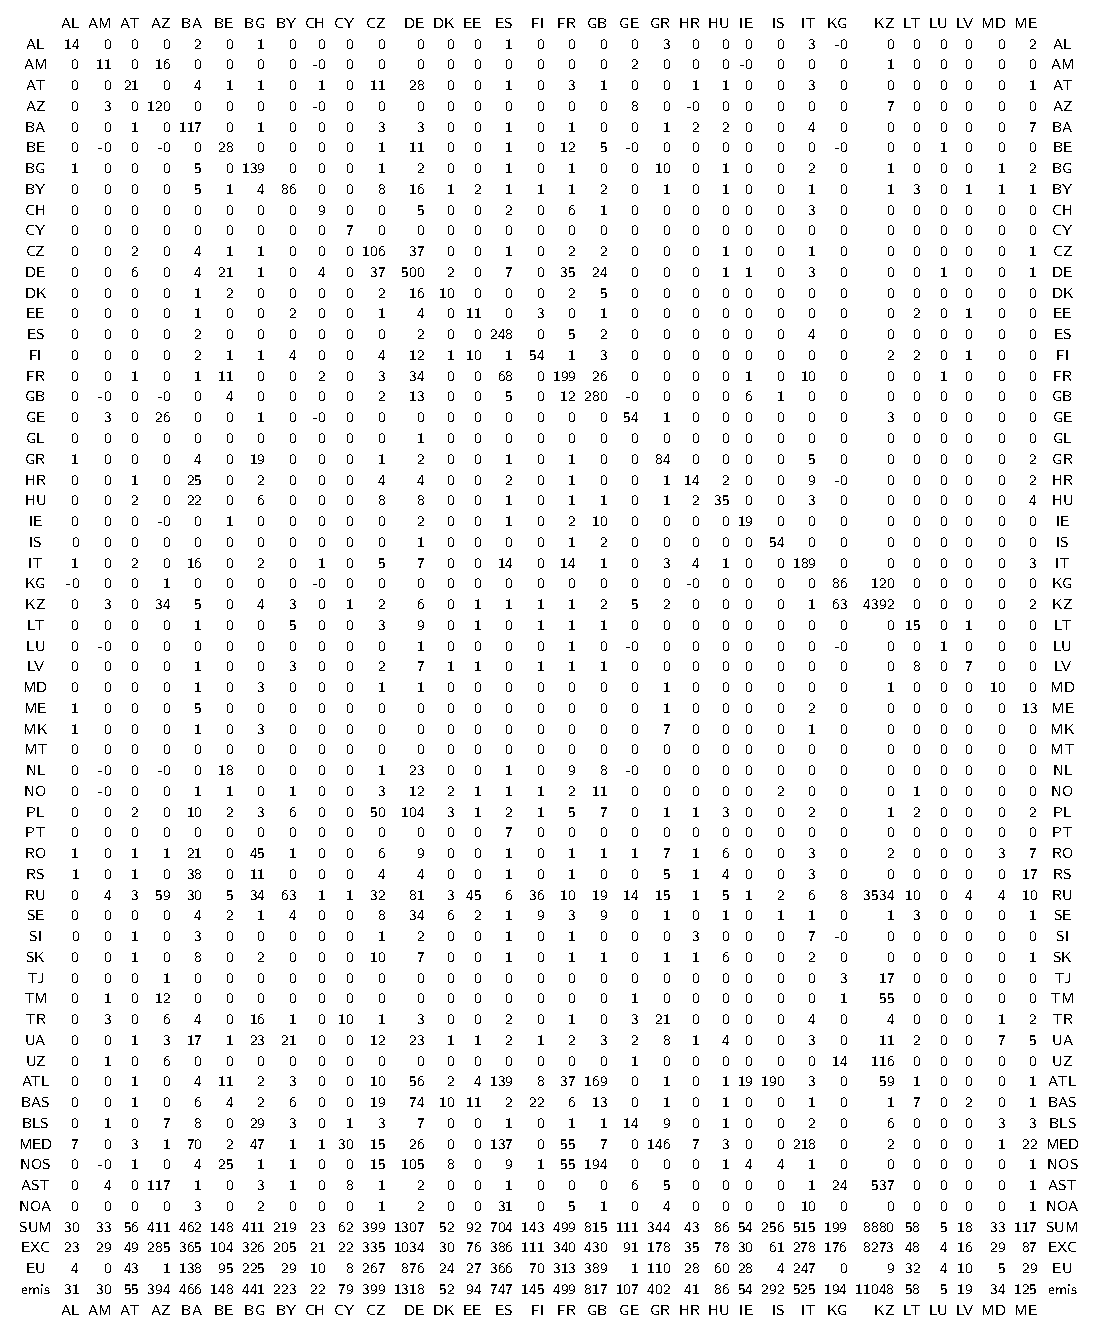
\epsfig{file=SR_Tables_2019/oxidised_sulphur_0.eps, width=\mywidth, height=\myheight}}\clearpage
\footnotesize{\mbox{Table \ref{ch:appx_sr2019}.1 Cont.: 2019
    country-to-country blame matrices for \textbf{oxidised sulphur}
    deposition.}\\ Units: 100 Mg of S. \textbf{Emitters
      $\rightarrow$, Receptors $\downarrow$}. }\\[\baselineskip]\enlargethispage{\myenlarge} \hspace{-0.5cm} 
\centerline{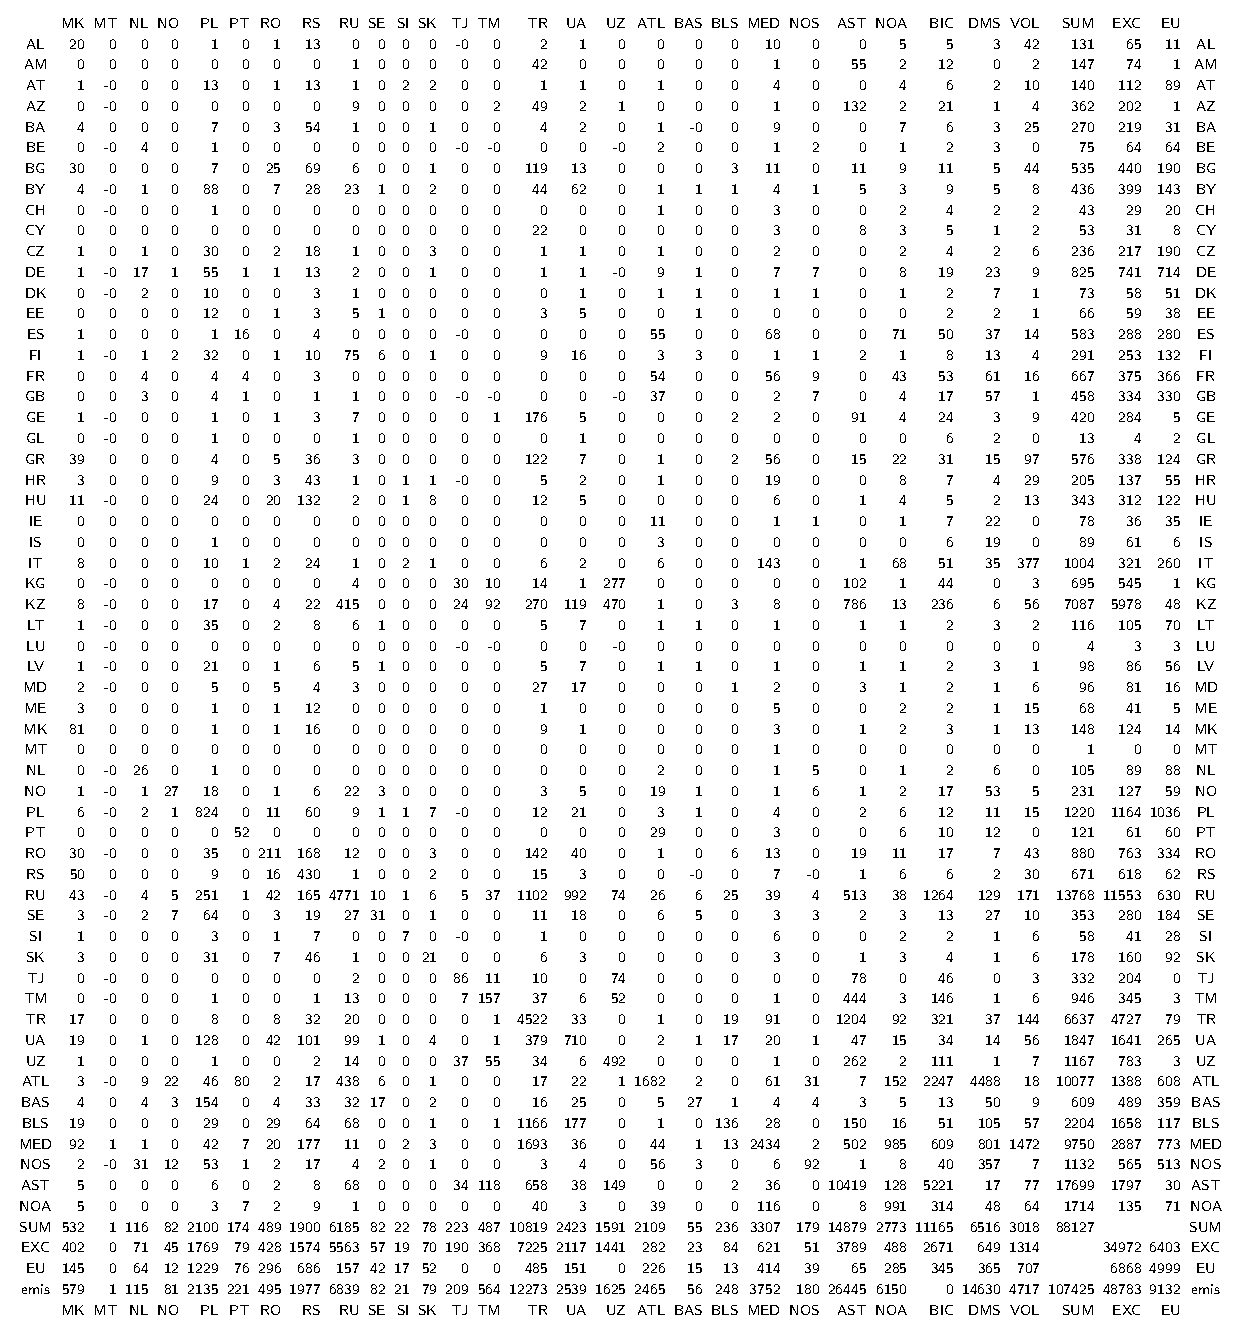
\epsfig{file=SR_Tables_2019/oxidised_sulphur_1.eps, width=\mywidth, height=\myheight}}\clearpage

% %table 2
\footnotesize{\mbox{Table \ref{ch:appx_sr2019}.2: 2019 country-to-country blame matrices for \textbf{oxidised nitrogen} deposition.}\\ Units: 100 Mg of N. \textbf{Emitters $\rightarrow$, Receptors $\downarrow$}. }\\[\baselineskip]\enlargethispage{\myenlarge} \hspace{-0.5cm} 
\centerline{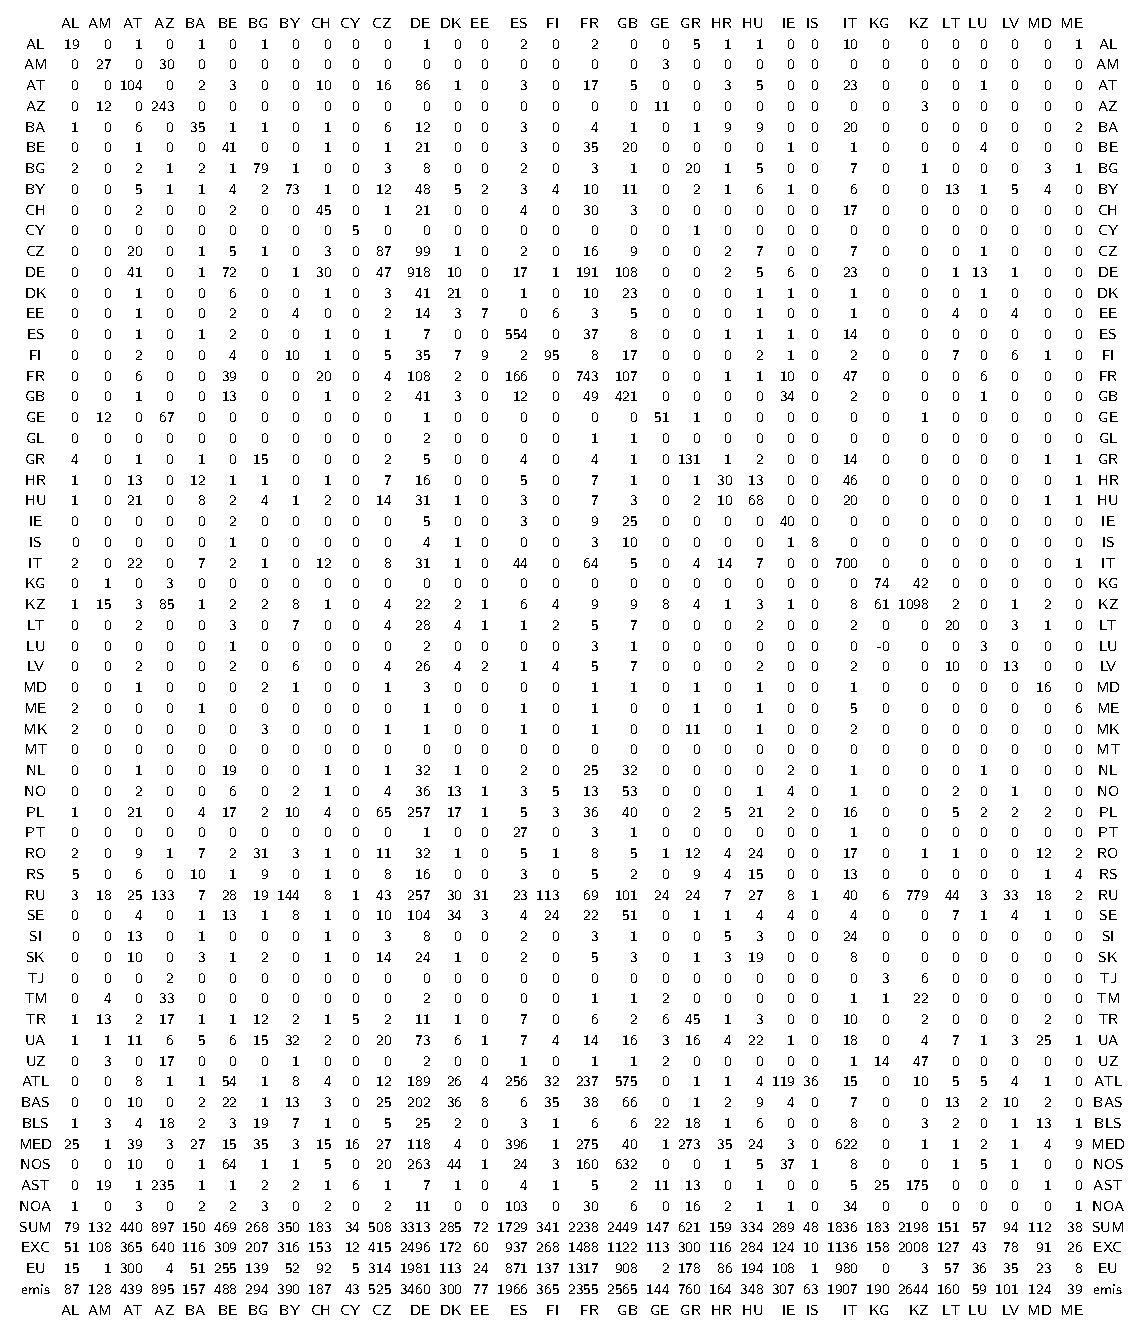
\epsfig{file=SR_Tables_2019/oxidised_nitrogen_0.eps, width=\mywidth, height=\myheight}}\clearpage
\footnotesize{\mbox{Table \ref{ch:appx_sr2019}.2 Cont.: 2019 country-to-country blame matrices for \textbf{oxidised nitrogen} deposition.}\\ Units: 100 Mg of N. \textbf{Emitters $\rightarrow$, Receptors $\downarrow$}. }\\[\baselineskip]\enlargethispage{\myenlarge} \hspace{-0.5cm} 
\centerline{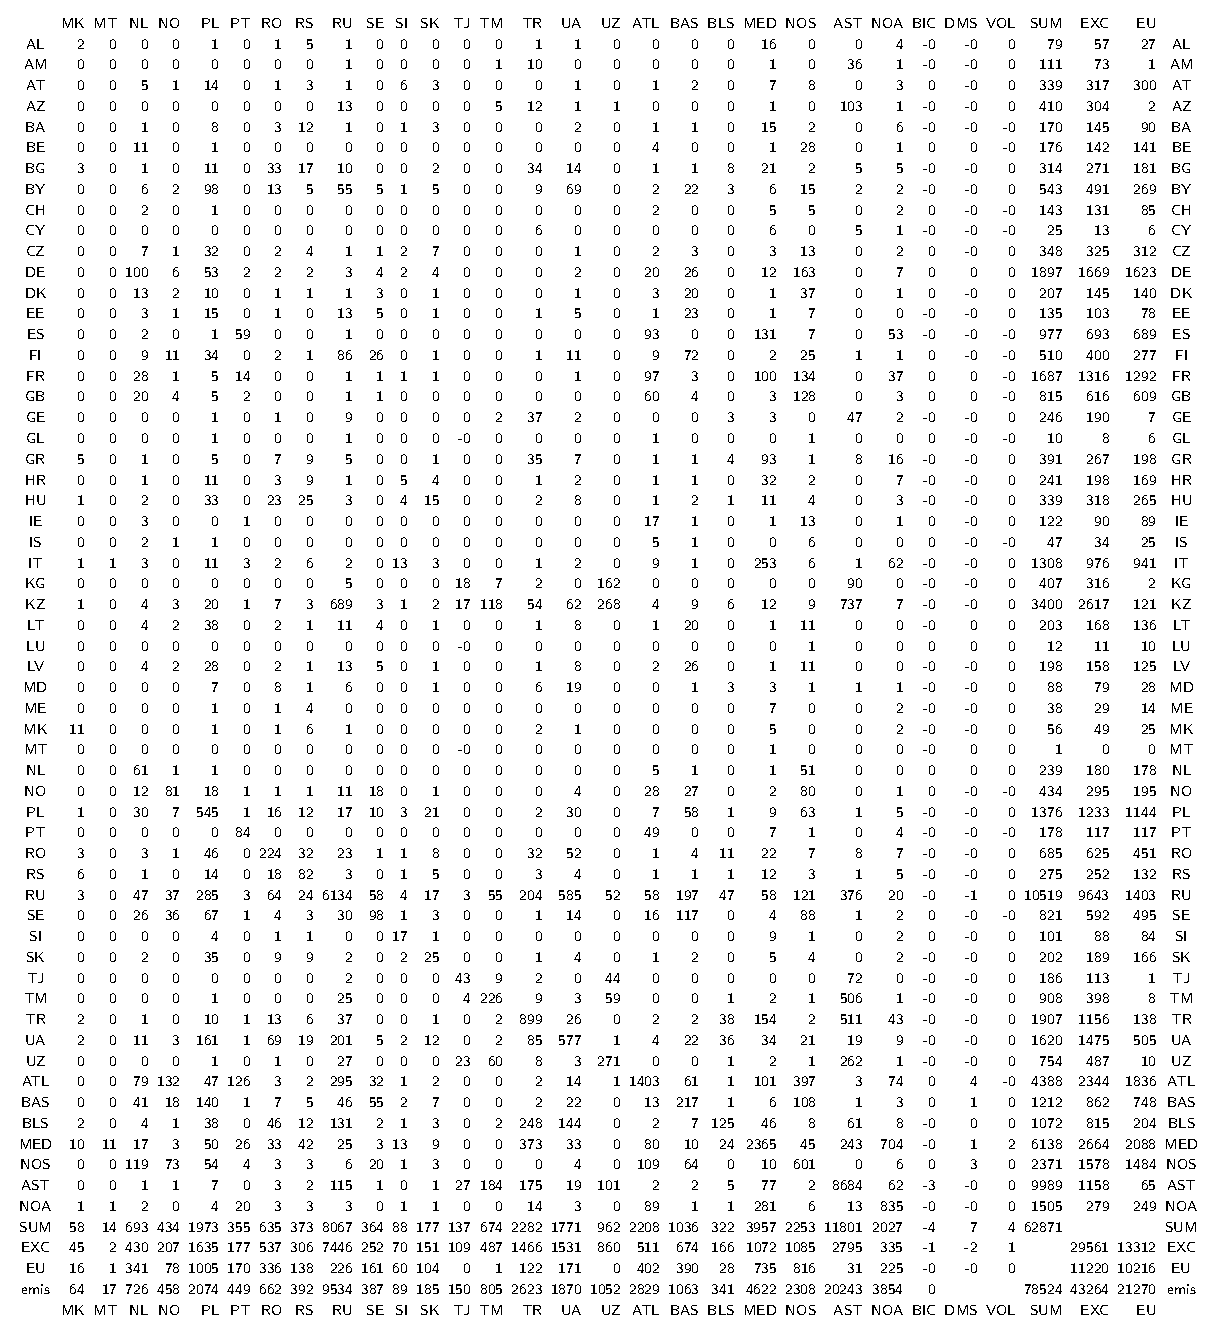
\epsfig{file=SR_Tables_2019/oxidised_nitrogen_1.eps, width=\mywidth, height=\myheight}}\clearpage

% %table 3
\footnotesize{\mbox{Table \ref{ch:appx_sr2019}.3: 2019 country-to-country blame matrices for \textbf{reduced nitrogen} deposition.}\\ Units: 100 Mg of N. \textbf{Emitters $\rightarrow$, Receptors $\downarrow$}. }\\[\baselineskip]\enlargethispage{\myenlarge} \hspace{-0.5cm} 
\centerline{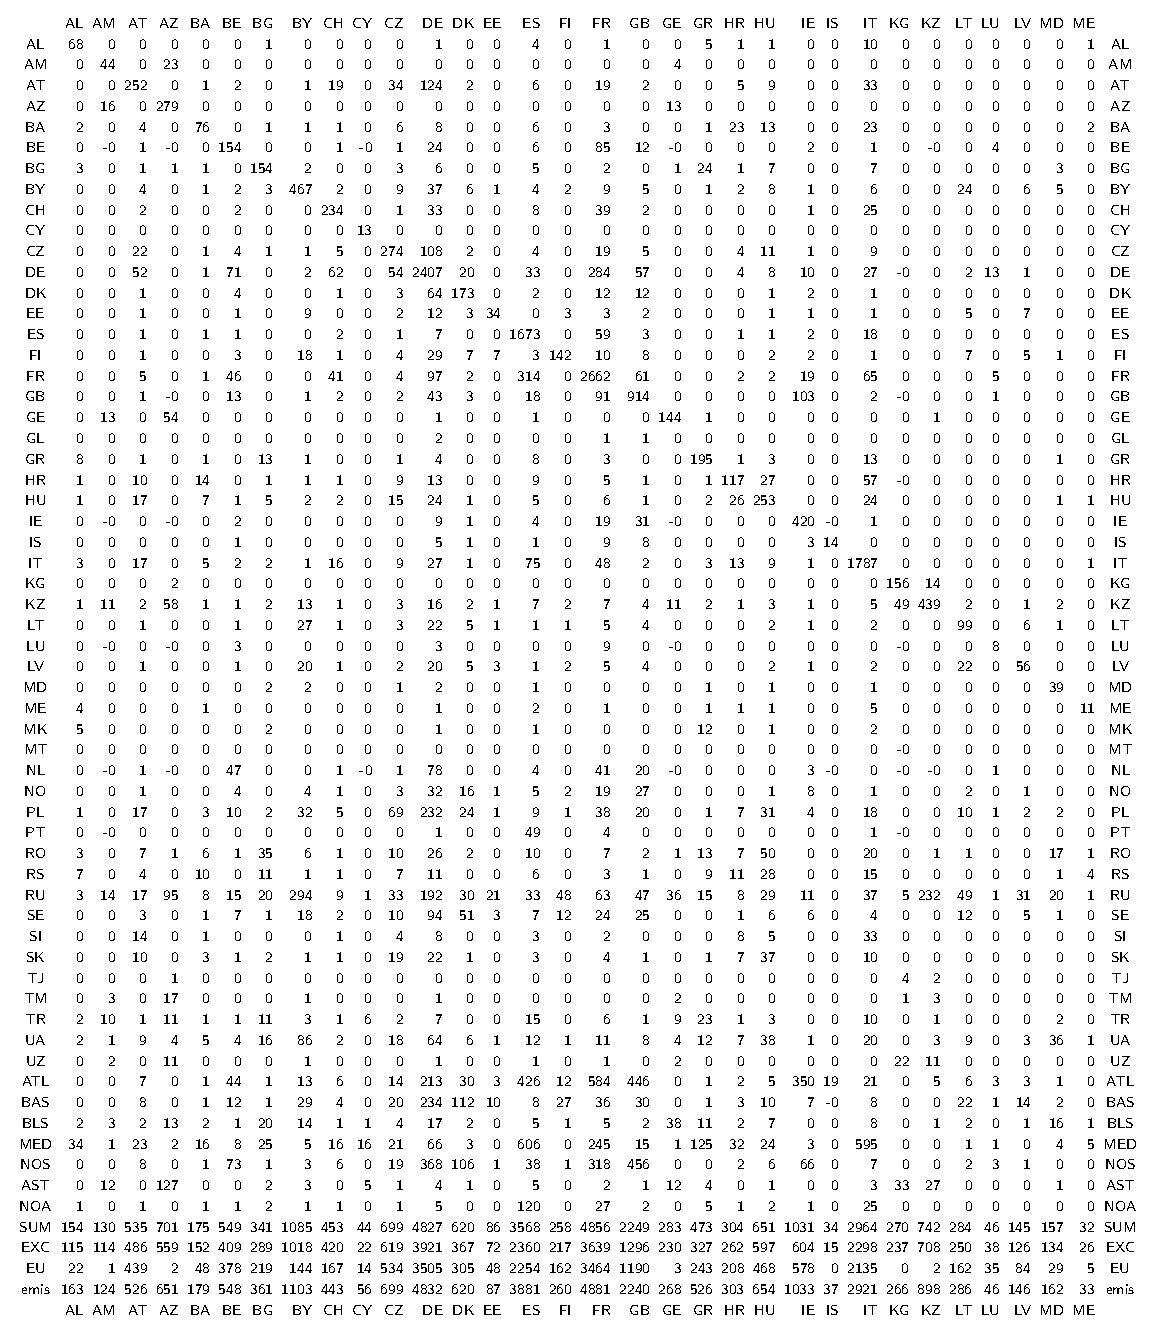
\epsfig{file=SR_Tables_2019/reduced_nitrogen_0.eps, width=\mywidth, height=\myheight}}\clearpage
\footnotesize{\mbox{Table \ref{ch:appx_sr2019}.3 Cont.: 2019 country-to-country blame matrices for \textbf{reduced nitrogen} deposition.}\\ Units: 100 Mg of N. \textbf{Emitters $\rightarrow$, Receptors $\downarrow$}. }\\[\baselineskip]\enlargethispage{\myenlarge} \hspace{-0.5cm} 
\centerline{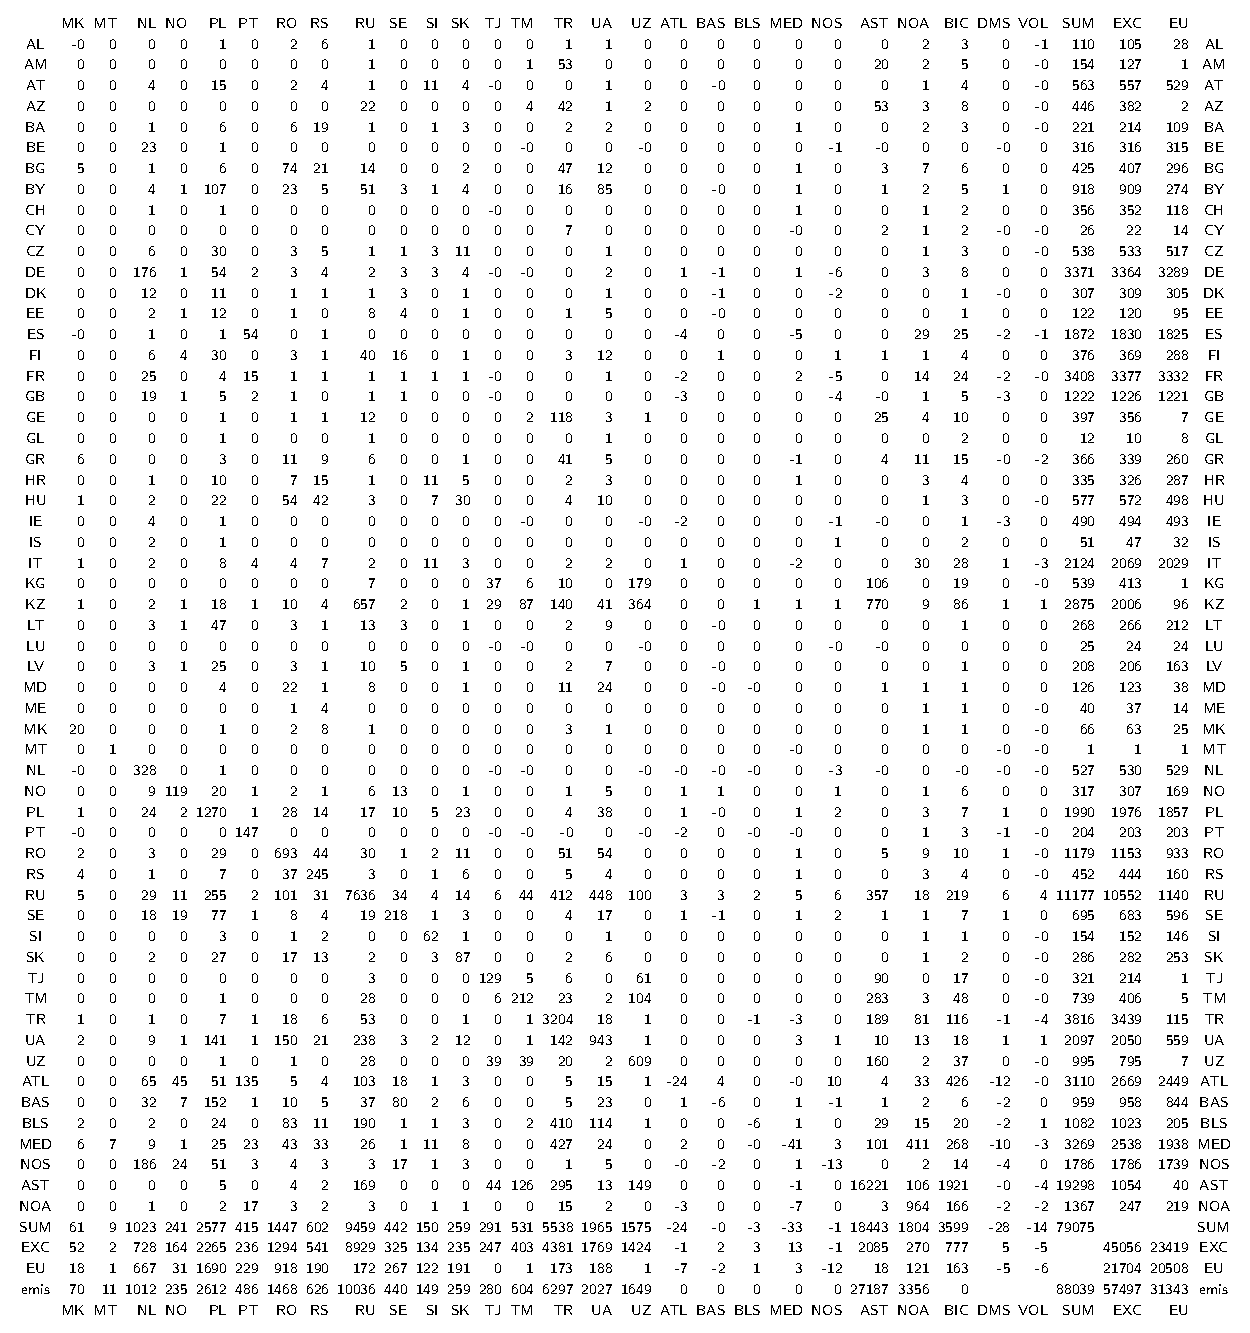
\epsfig{file=SR_Tables_2019/reduced_nitrogen_1.eps, width=\mywidth, height=\myheight}}\clearpage

% %table 4
\footnotesize{\mbox{Table \ref{ch:appx_sr2019}.4: 2019 country-to-country blame matrices for \textbf{\aotucf}.}\\ Units: ppb.h per 15\% emis. red. of NO$_x$. \textbf{Emitters $\rightarrow$, Receptors $\downarrow$}. }\\[\baselineskip]\enlargethispage{\myenlarge} \hspace{-0.5cm} 
\centerline{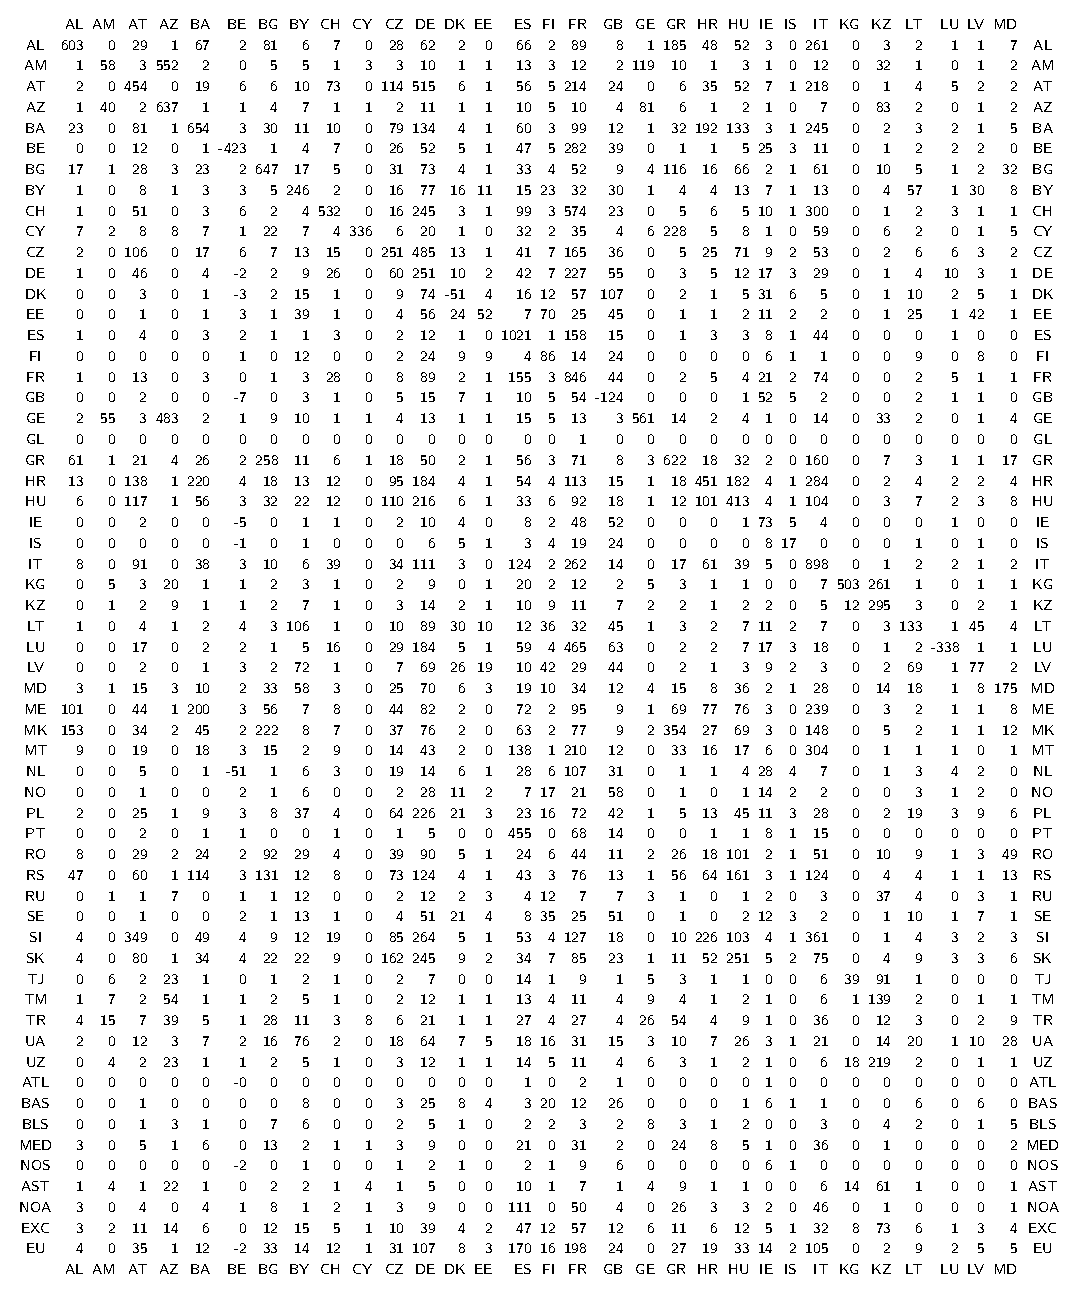
\epsfig{file=SR_Tables_2019/AOT40df_NOx_0.eps, width=\mywidth, height=\myheight}}\clearpage
\footnotesize{\mbox{Table \ref{ch:appx_sr2019}.4 Cont.: 2019 country-to-country blame matrices for \textbf{\aotucf}.}\\ Units: ppb.h per 15\% emis. red. of NO$_x$. \textbf{Emitters $\rightarrow$, Receptors $\downarrow$}. }\\[\baselineskip]\enlargethispage{\myenlarge} \hspace{-0.5cm} 
\centerline{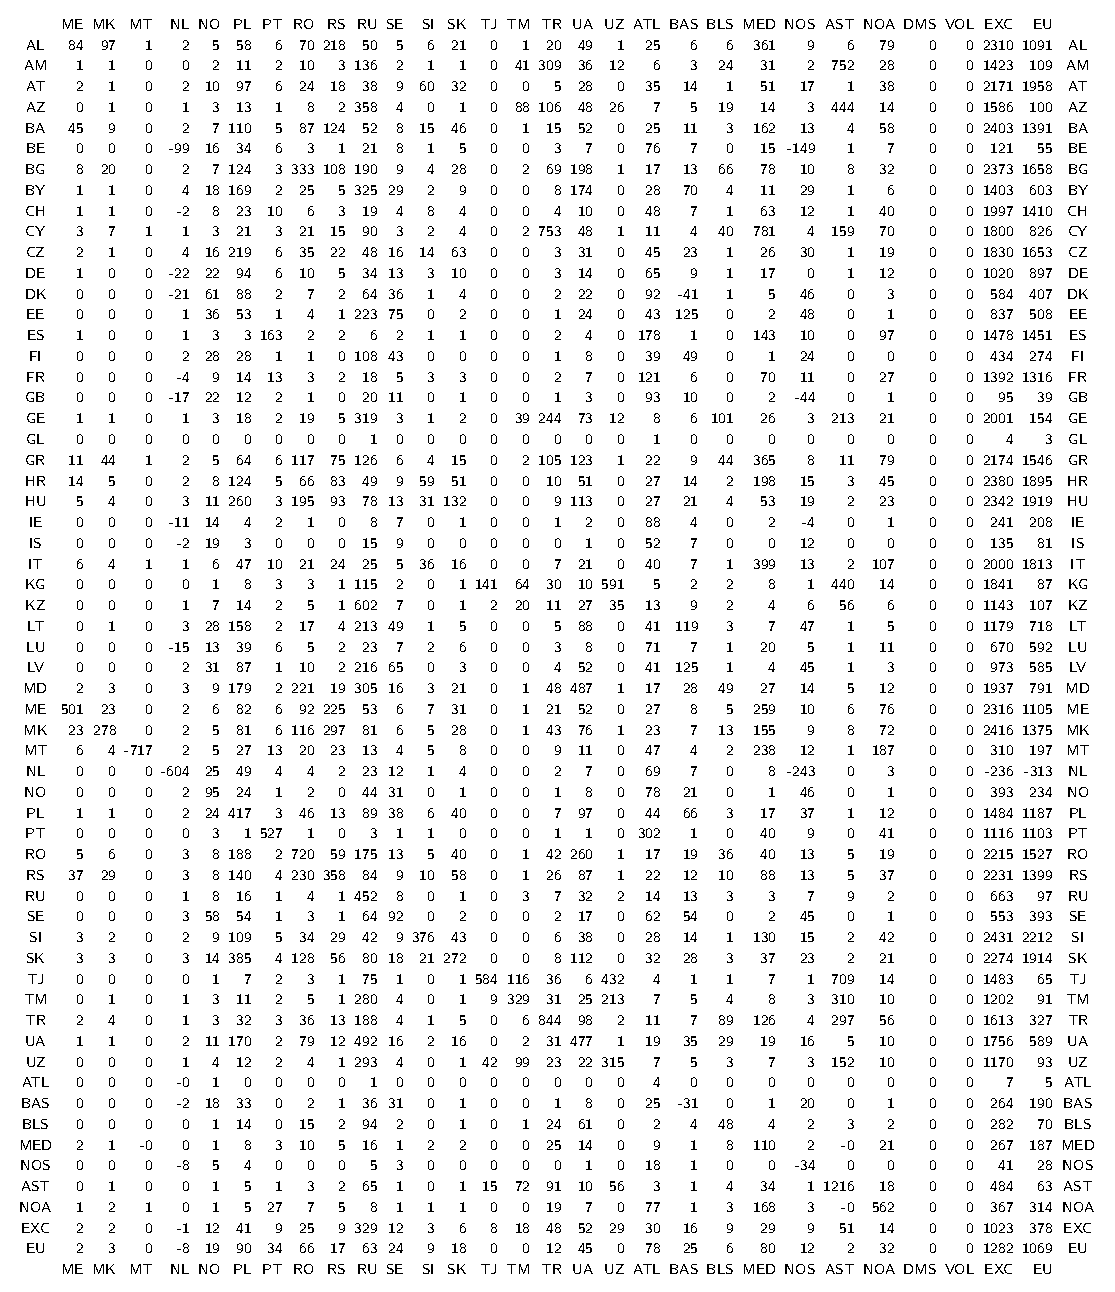
\epsfig{file=SR_Tables_2019/AOT40df_NOx_1.eps, width=\mywidth, height=\myheight}}\clearpage

% %table 5
\footnotesize{\mbox{Table \ref{ch:appx_sr2019}.5: 2019 country-to-country blame matrices for \textbf{\aotucf}.}\\ Units: ppb.h per 15\% emis. red. of VOC. \textbf{Emitters $\rightarrow$, Receptors $\downarrow$}. }\\[\baselineskip]\enlargethispage{\myenlarge} \hspace{-0.5cm} 
\centerline{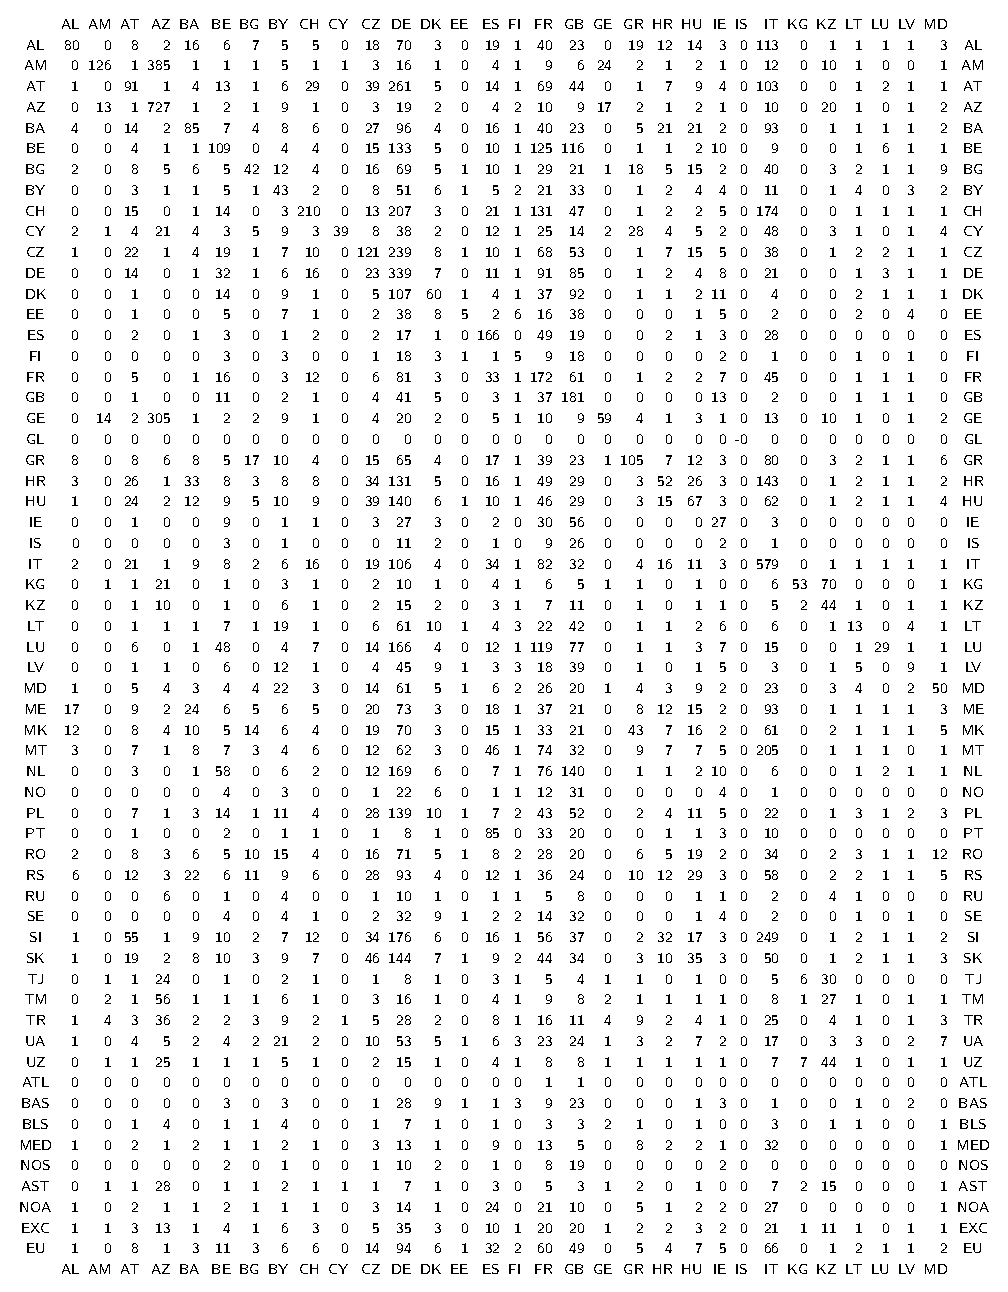
\epsfig{file=SR_Tables_2019/AOT40df_NMVOC_0.eps, width=\mywidth, height=\myheight}}\clearpage
\footnotesize{\mbox{Table \ref{ch:appx_sr2019}.5 Cont.: 2019 country-to-country blame matrices for \textbf{\aotucf}.}\\ Units: ppb.h per 15\% emis. red. of VOC. \textbf{Emitters $\rightarrow$, Receptors $\downarrow$}. }\\[\baselineskip]\enlargethispage{\myenlarge} \hspace{-0.5cm} 
\centerline{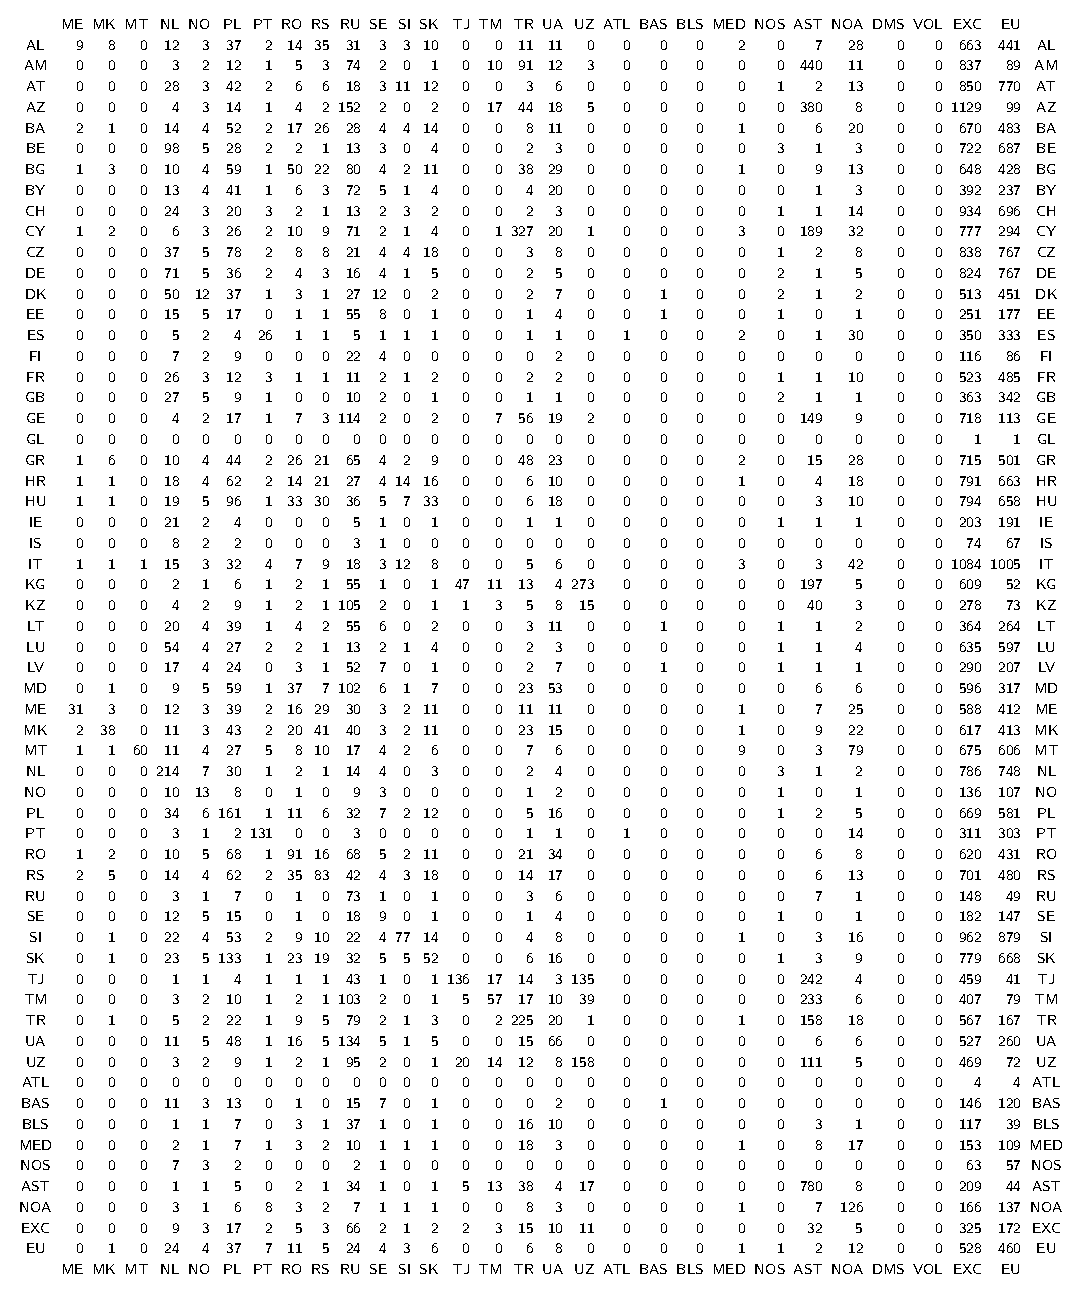
\epsfig{file=SR_Tables_2019/AOT40df_NMVOC_1.eps, width=\mywidth, height=\myheight}}\clearpage

% %table 6
\footnotesize{\mbox{Table \ref{ch:appx_sr2019}.6: 2019 country-to-country blame matrices for \textbf{SOMO35}.}\\ Units: ppb.d per 15\% emis. red. of NO$_x$. \textbf{Emitters $\rightarrow$, Receptors $\downarrow$}. }\\[\baselineskip]\enlargethispage{\myenlarge} \hspace{-0.5cm} 
\centerline{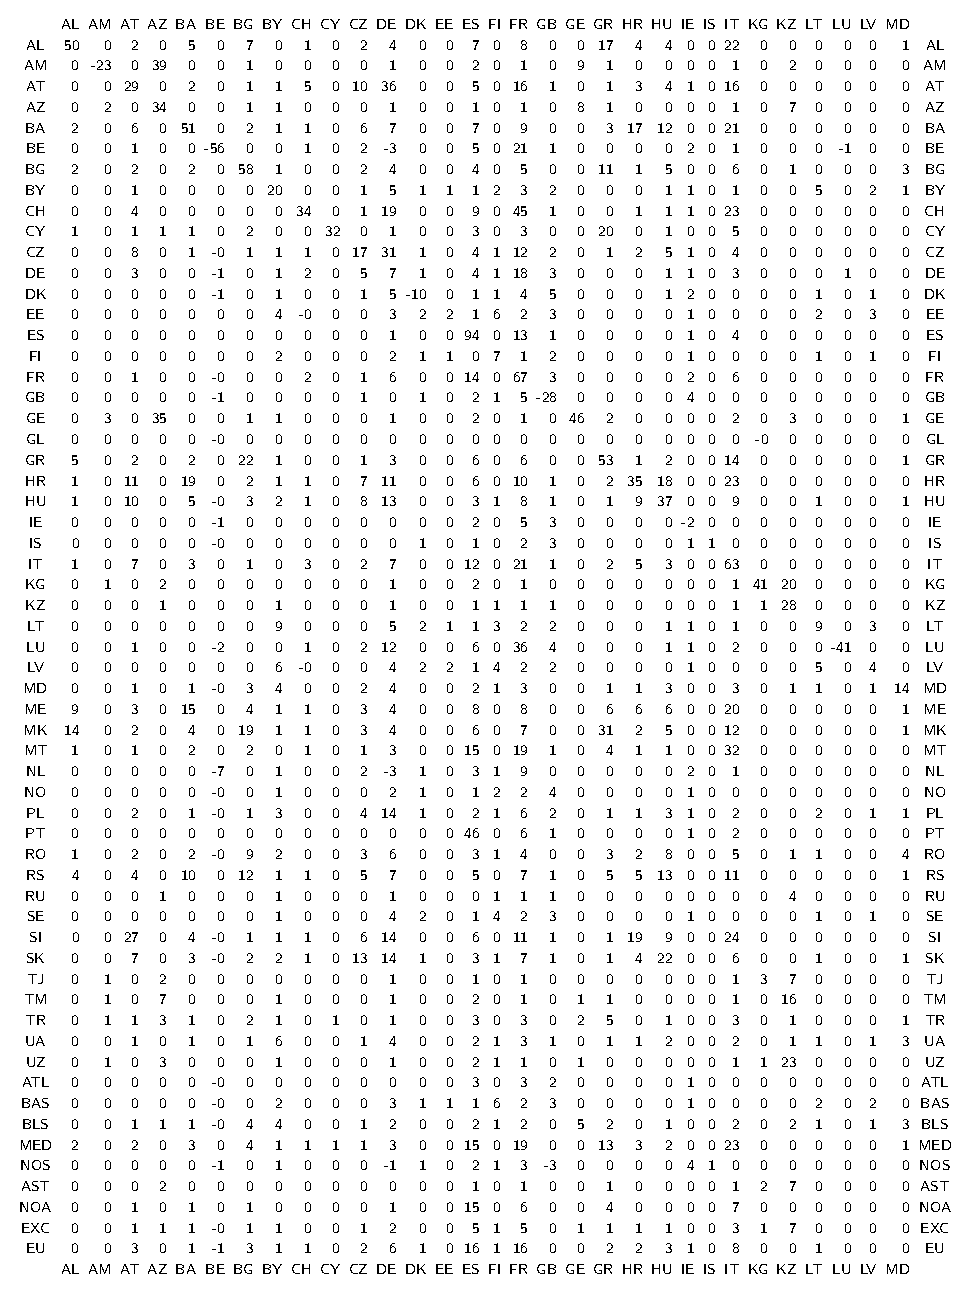
\epsfig{file=SR_Tables_2019/SOMO35_NOx_0.eps, width=\mywidth, height=\myheight}}\clearpage
\footnotesize{\mbox{Table \ref{ch:appx_sr2019}.6 Cont.: 2019 country-to-country blame matrices for \textbf{SOMO35}.}\\ Units: ppb.d per 15\% emis. red. of NO$_x$. \textbf{Emitters $\rightarrow$, Receptors $\downarrow$}. }\\[\baselineskip]\enlargethispage{\myenlarge} \hspace{-0.5cm} 
\centerline{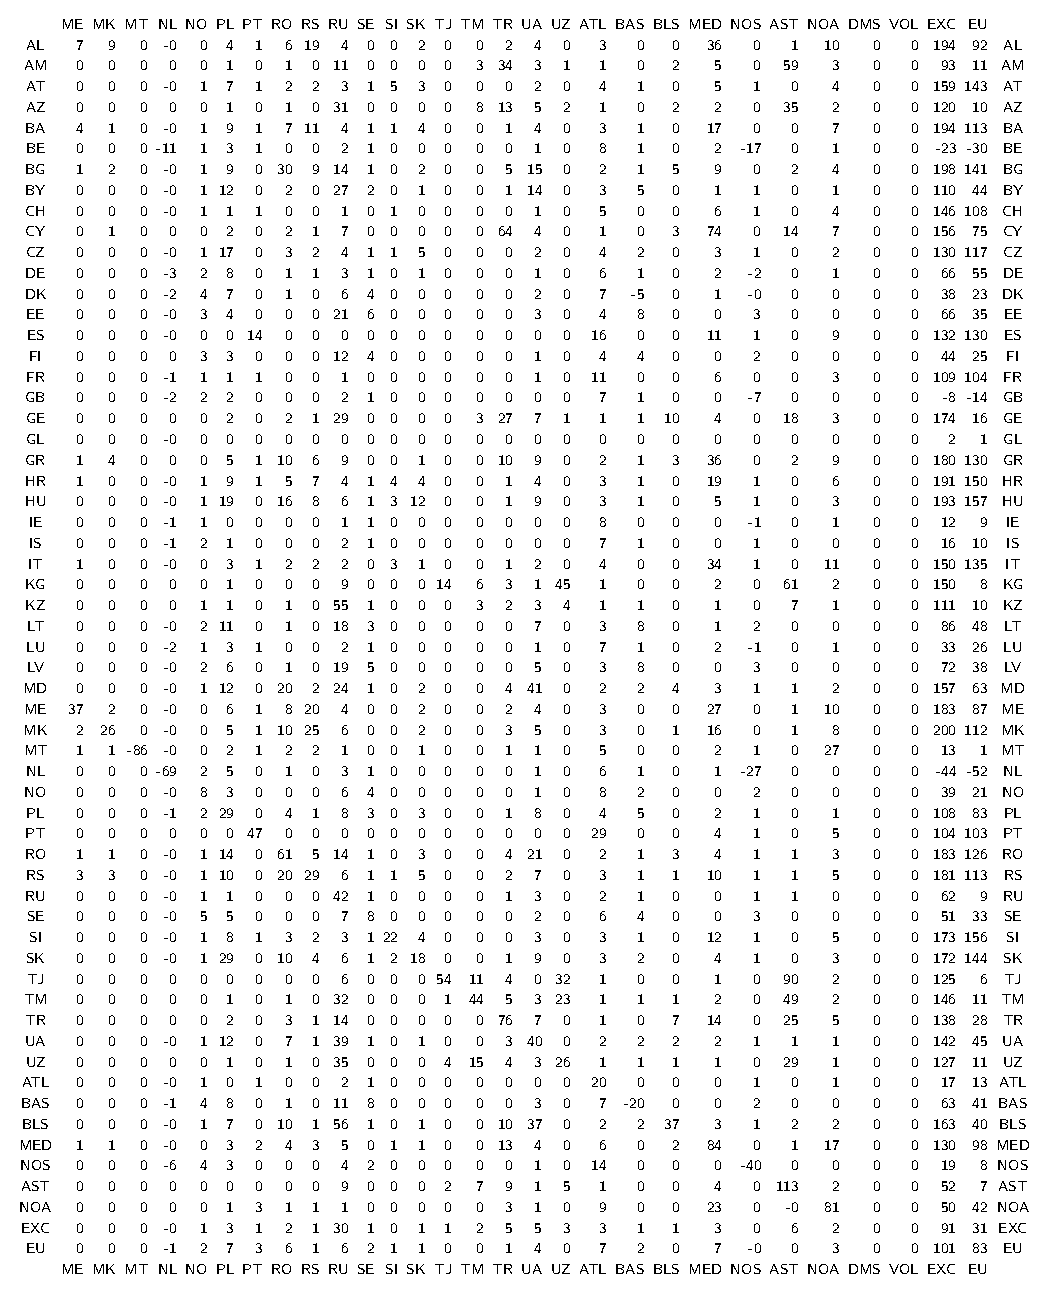
\epsfig{file=SR_Tables_2019/SOMO35_NOx_1.eps, width=\mywidth, height=\myheight}}\clearpage

% %table 7
\footnotesize{\mbox{Table \ref{ch:appx_sr2019}.7: 2019 country-to-country blame matrices for \textbf{SOMO35}.}\\ Units: ppb.d per 15\% emis. red. of VOC. \textbf{Emitters $\rightarrow$, Receptors $\downarrow$}. }\\[\baselineskip]\enlargethispage{\myenlarge} \hspace{-0.5cm} 
\centerline{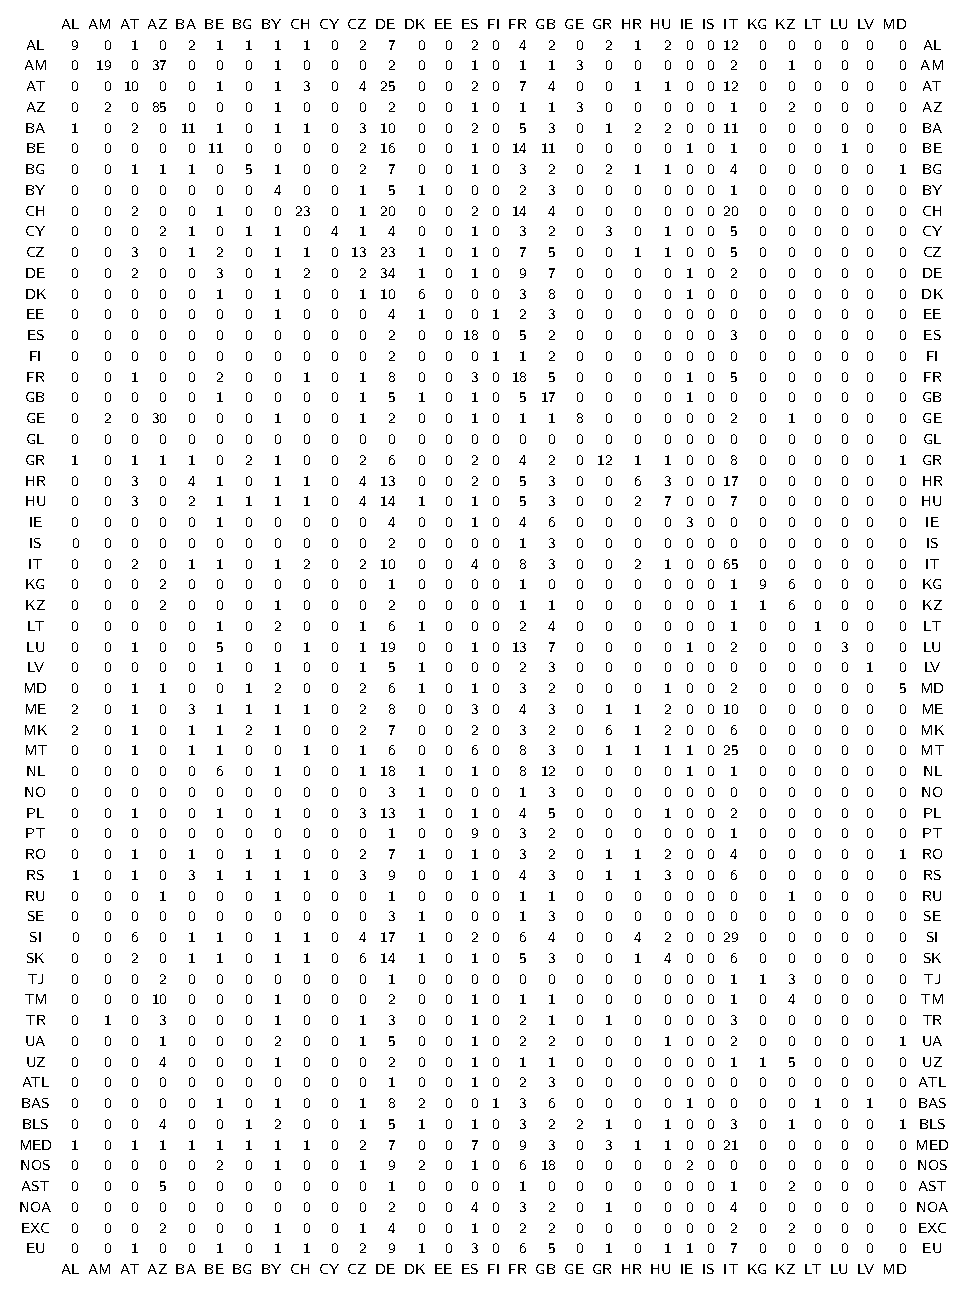
\epsfig{file=SR_Tables_2019/SOMO35_NMVOC_0.eps, width=\mywidth, height=\myheight}}\clearpage
\footnotesize{\mbox{Table \ref{ch:appx_sr2019}.7 Cont.: 2019 country-to-country blame matrices for \textbf{SOMO35}.}\\ Units: ppb.d per 15\% emis. red. of VOC. \textbf{Emitters $\rightarrow$, Receptors $\downarrow$}. }\\[\baselineskip]\enlargethispage{\myenlarge} \hspace{-0.5cm} 
\centerline{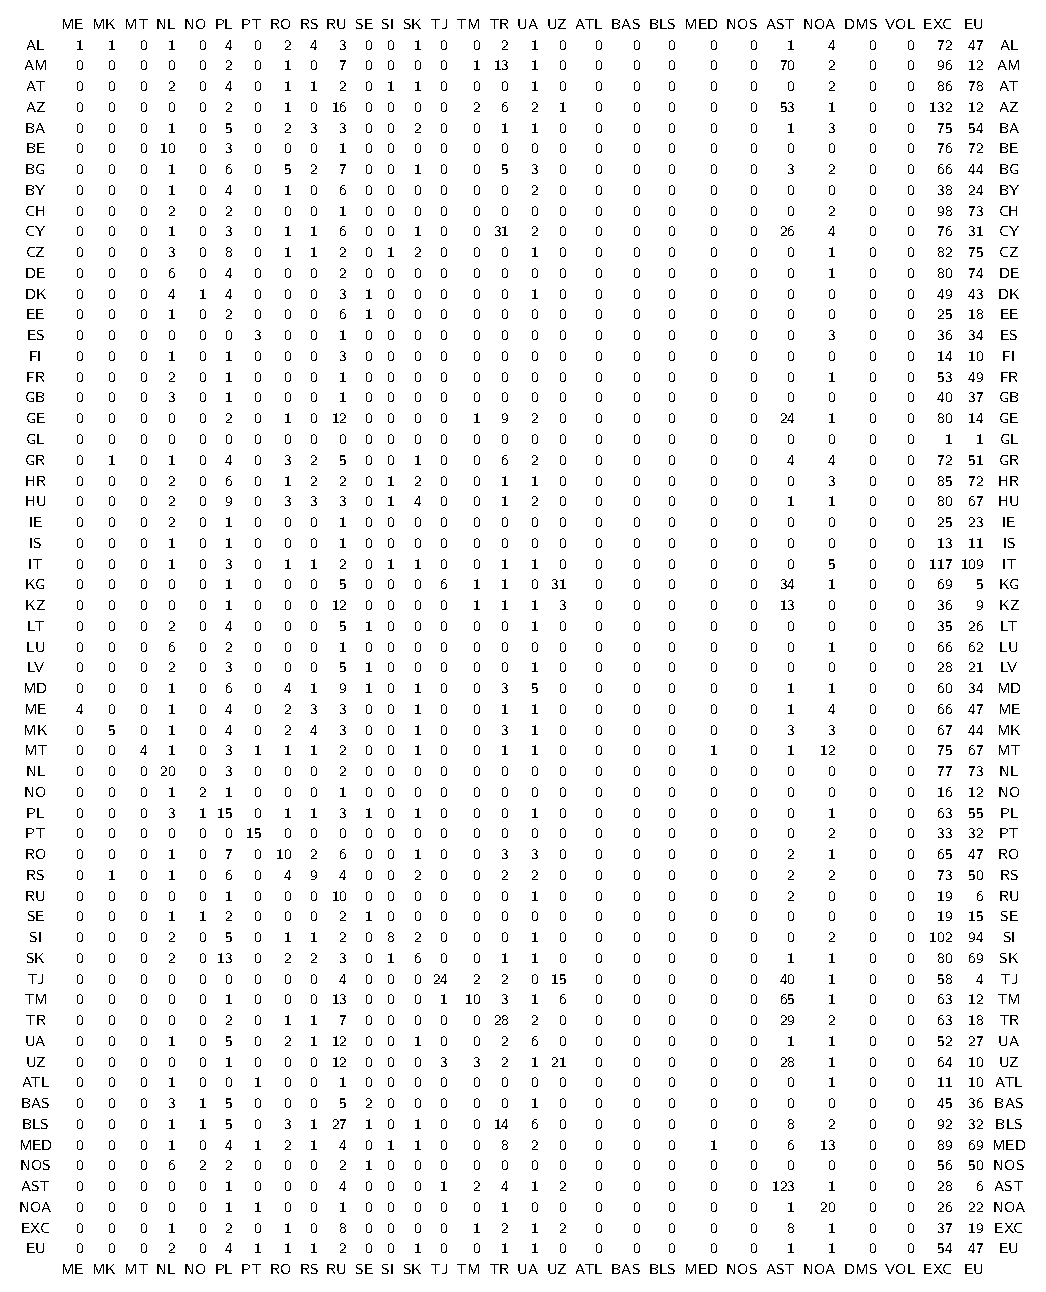
\epsfig{file=SR_Tables_2019/SOMO35_NMVOC_1.eps, width=\mywidth, height=\myheight}}\clearpage

% %table 8
\footnotesize{\mbox{Table \ref{ch:appx_sr2019}.8: 2019 country-to-country blame matrices for \textbf{PM2.5}.}\\ Units: ng/m$^3$ per 15\% emis. red. of PPM. \textbf{Emitters $\rightarrow$, Receptors $\downarrow$}. }\\[\baselineskip]\enlargethispage{\myenlarge} \hspace{-0.5cm} 
\centerline{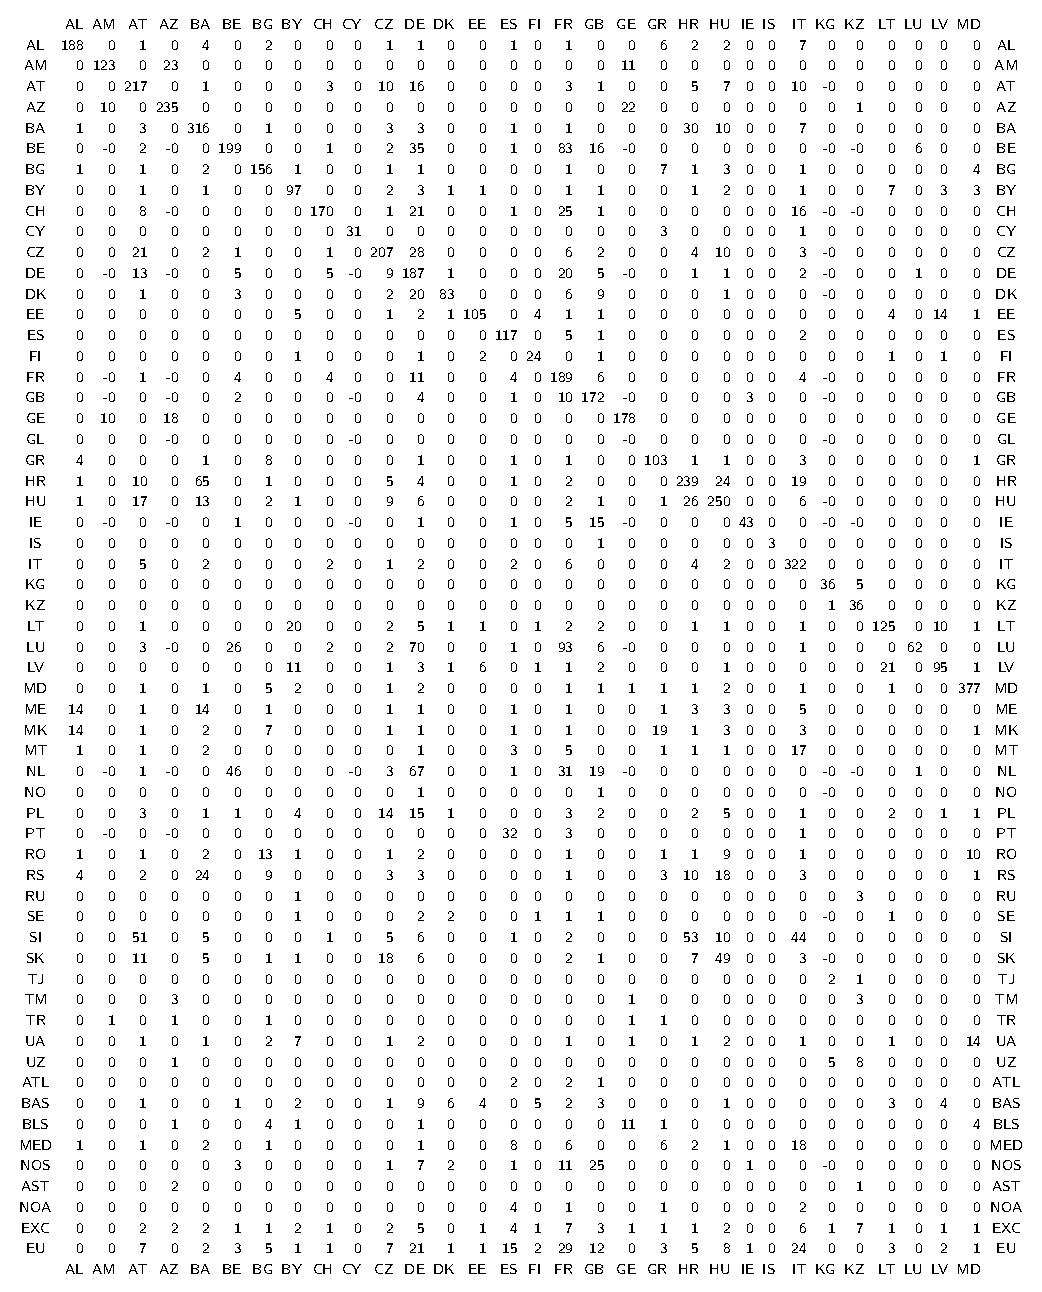
\epsfig{file=SR_Tables_2019/PM25_PPM_0.eps, width=\mywidth, height=\myheight}}\clearpage
\footnotesize{\mbox{Table \ref{ch:appx_sr2019}.8 Cont.: 2019 country-to-country blame matrices for \textbf{PM2.5}.}\\ Units: ng/m$^3$ per 15\% emis. red. of PPM. \textbf{Emitters $\rightarrow$, Receptors $\downarrow$}. }\\[\baselineskip]\enlargethispage{\myenlarge} \hspace{-0.5cm} 
\centerline{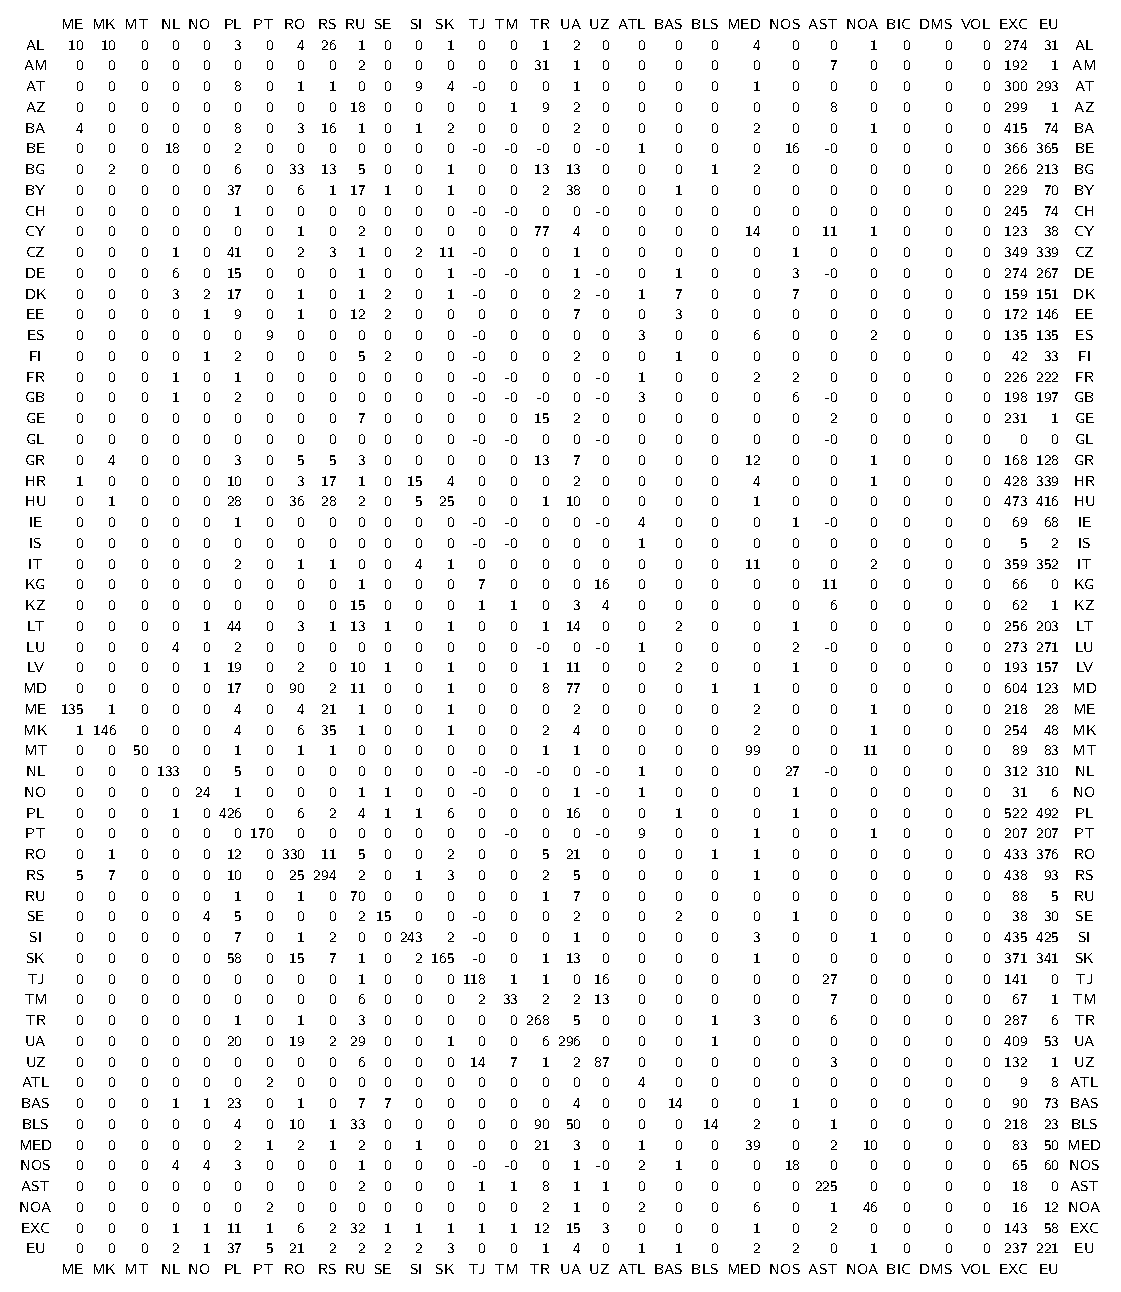
\epsfig{file=SR_Tables_2019/PM25_PPM_1.eps, width=\mywidth, height=\myheight}}\clearpage

% % table 9
\footnotesize{\mbox{Table \ref{ch:appx_sr2019}.9: 2019 country-to-country blame matrices for \textbf{PM2.5}.}\\ Units: ng/m$^3$ per 15\% emis. red. of SO$_x$. \textbf{Emitters $\rightarrow$, Receptors $\downarrow$}. }\\[\baselineskip]\enlargethispage{\myenlarge} \hspace{-0.5cm} 
\centerline{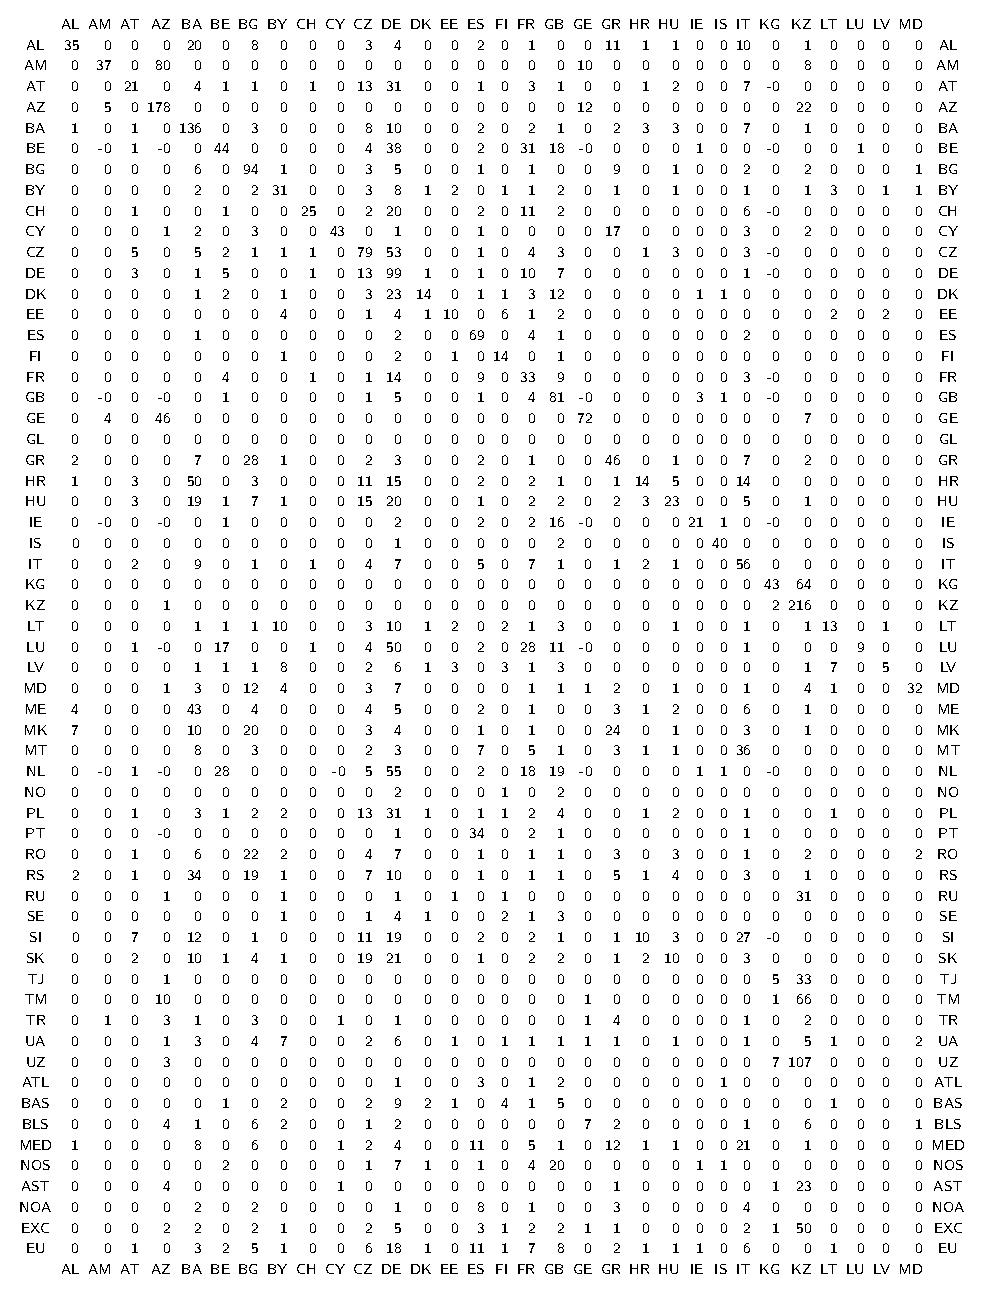
\epsfig{file=SR_Tables_2019/PM25_SOx_0.eps, width=\mywidth, height=\myheight}}\clearpage
\footnotesize{\mbox{Table \ref{ch:appx_sr2019}.9 Cont.: 2019 country-to-country blame matrices for \textbf{PM2.5}.}\\ Units: ng/m$^3$ per 15\% emis. red. of SO$_x$. \textbf{Emitters $\rightarrow$, Receptors $\downarrow$}. }\\[\baselineskip]\enlargethispage{\myenlarge} \hspace{-0.5cm} 
\centerline{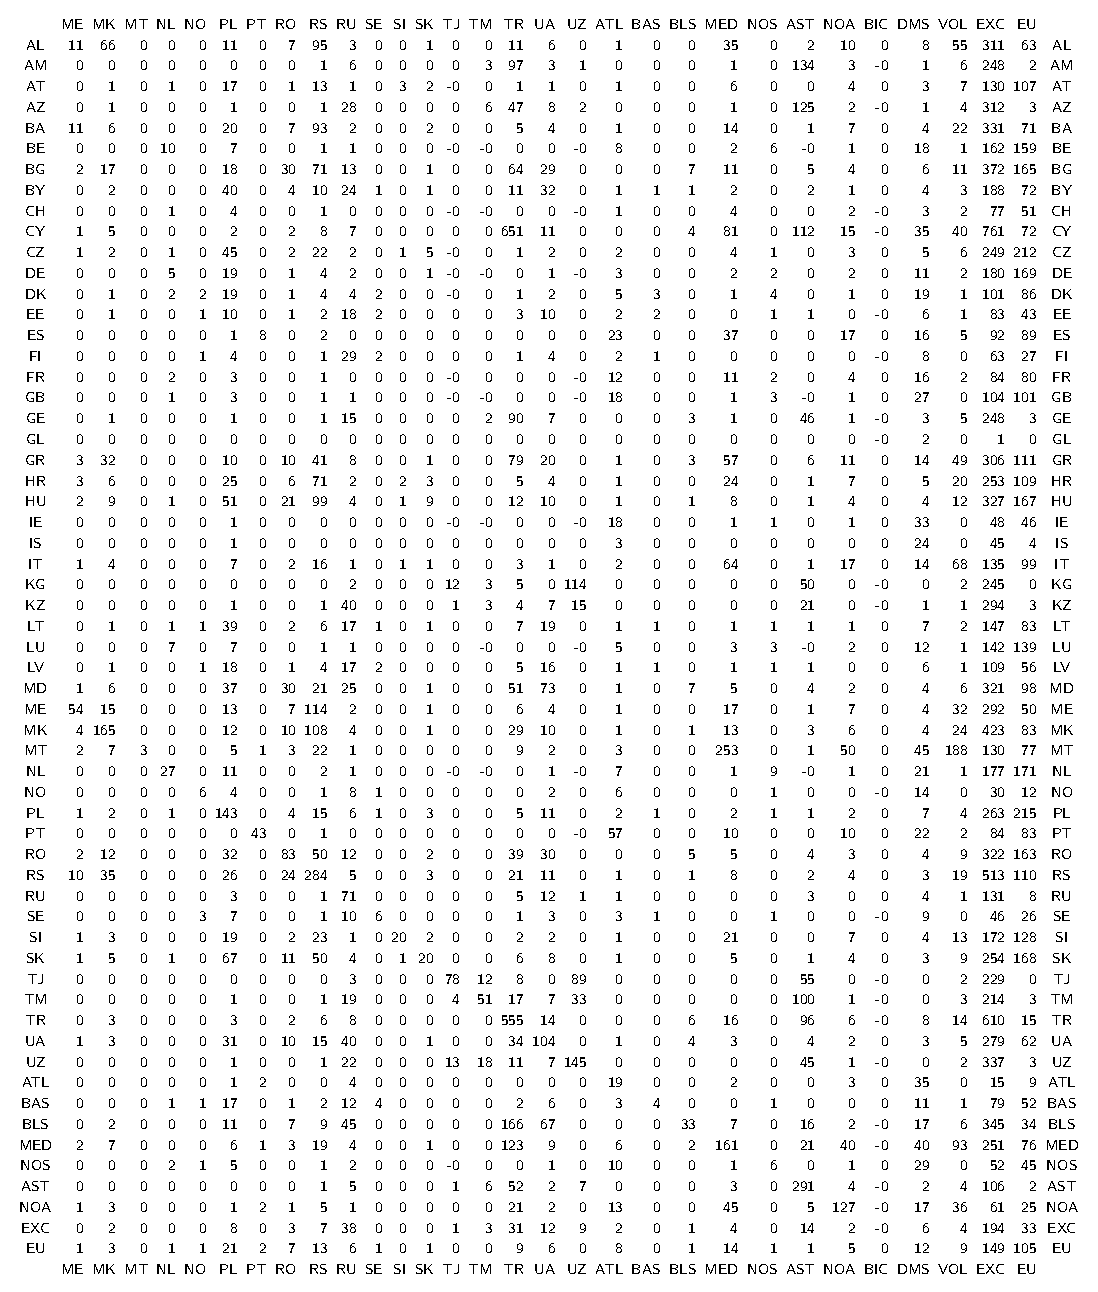
\epsfig{file=SR_Tables_2019/PM25_SOx_1.eps, width=\mywidth, height=\myheight}}\clearpage

% % table 10
\footnotesize{\mbox{Table \ref{ch:appx_sr2019}.10: 2019 country-to-country blame matrices for \textbf{PM2.5}.}\\ Units: ng/m$^3$ per 15\% emis. red. of NO$_x$. \textbf{Emitters $\rightarrow$, Receptors $\downarrow$}. }\\[\baselineskip]\enlargethispage{\myenlarge} \hspace{-0.5cm} 
\centerline{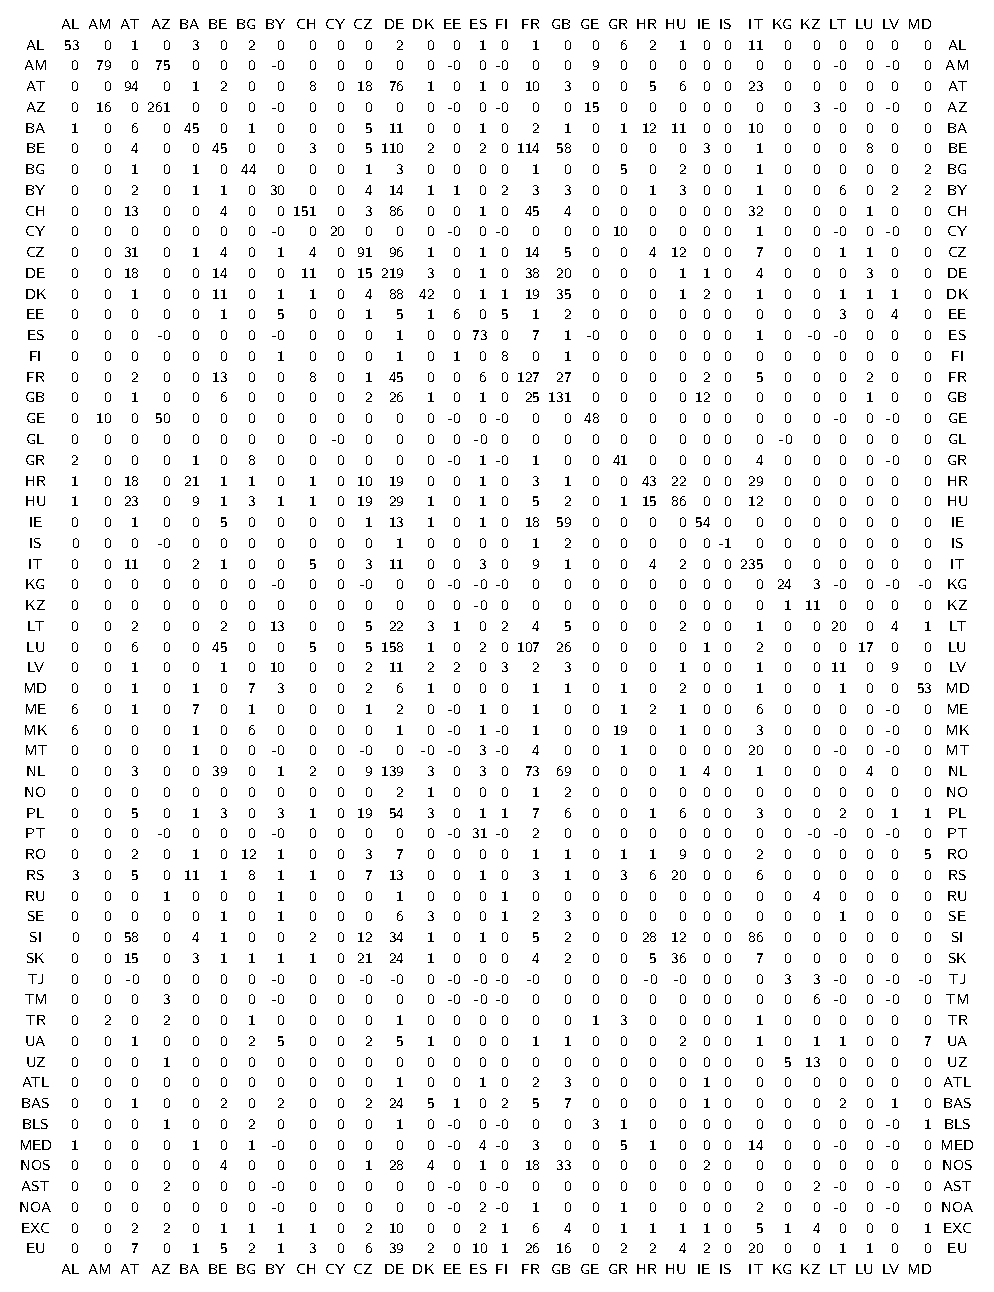
\epsfig{file=SR_Tables_2019/PM25_NOx_0.eps, width=\mywidth, height=\myheight}}\clearpage
\footnotesize{\mbox{Table \ref{ch:appx_sr2019}.10 Cont.: 2019 country-to-country blame matrices for \textbf{PM2.5}.}\\ Units: ng/m$^3$ per 15\% emis. red. of NO$_x$. \textbf{Emitters $\rightarrow$, Receptors $\downarrow$}. }\\[\baselineskip]\enlargethispage{\myenlarge} \hspace{-0.5cm} 
\centerline{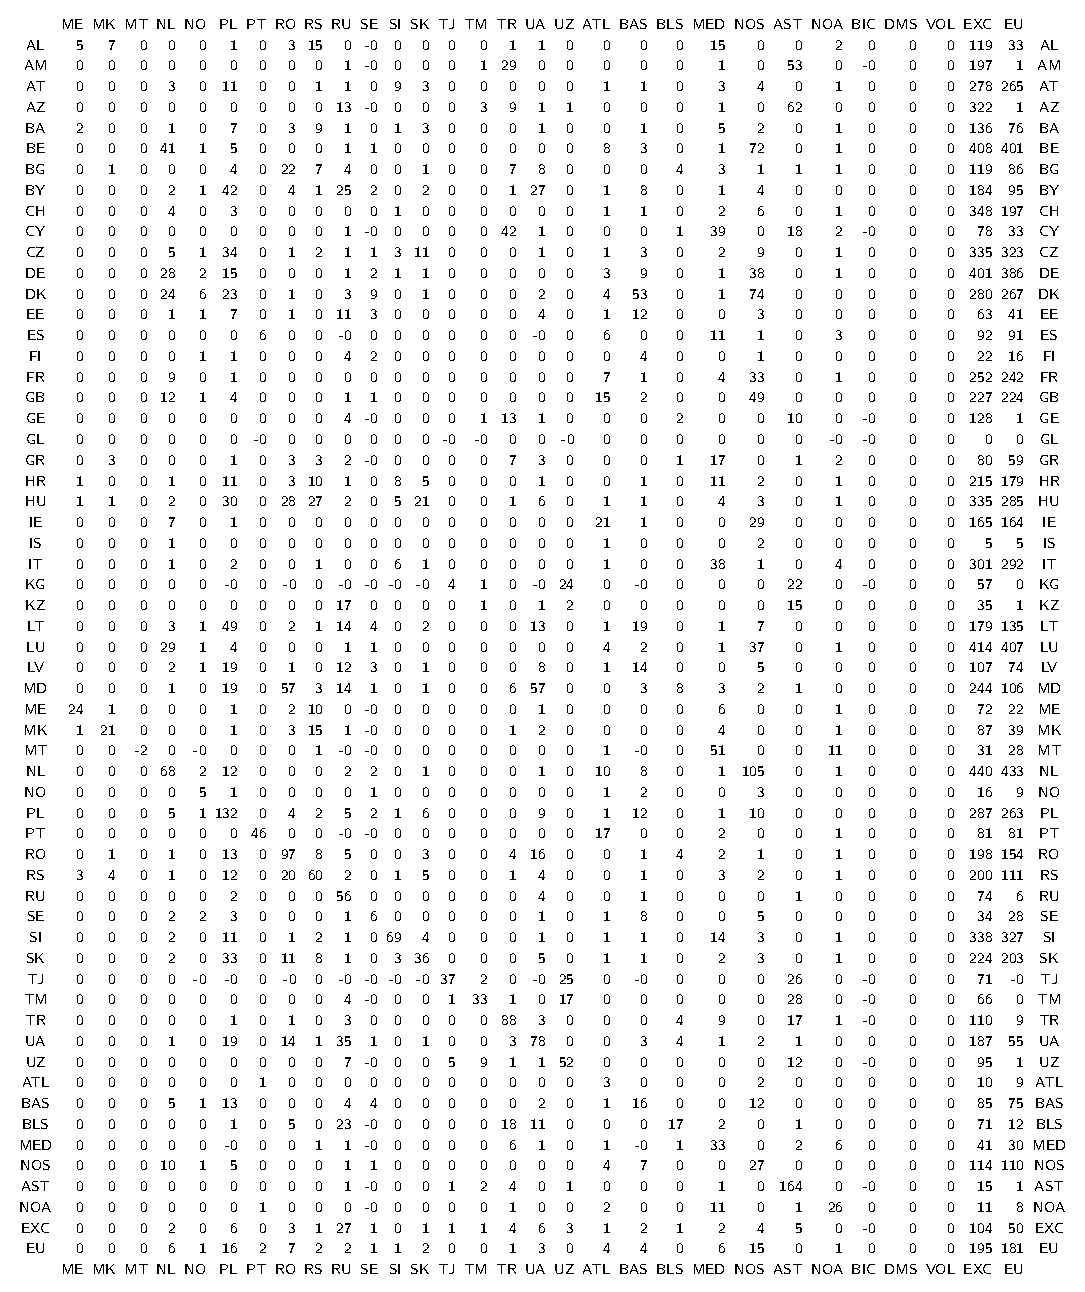
\epsfig{file=SR_Tables_2019/PM25_NOx_1.eps, width=\mywidth, height=\myheight}}\clearpage

% % table 11
\footnotesize{\mbox{Table \ref{ch:appx_sr2019}.11: 2019 country-to-country blame matrices for \textbf{PM2.5}.}\\ Units: ng/m$^3$ per 15\% emis. red. of NH$_3$. \textbf{Emitters $\rightarrow$, Receptors $\downarrow$}. }\\[\baselineskip]\enlargethispage{\myenlarge} \hspace{-0.5cm} 
\centerline{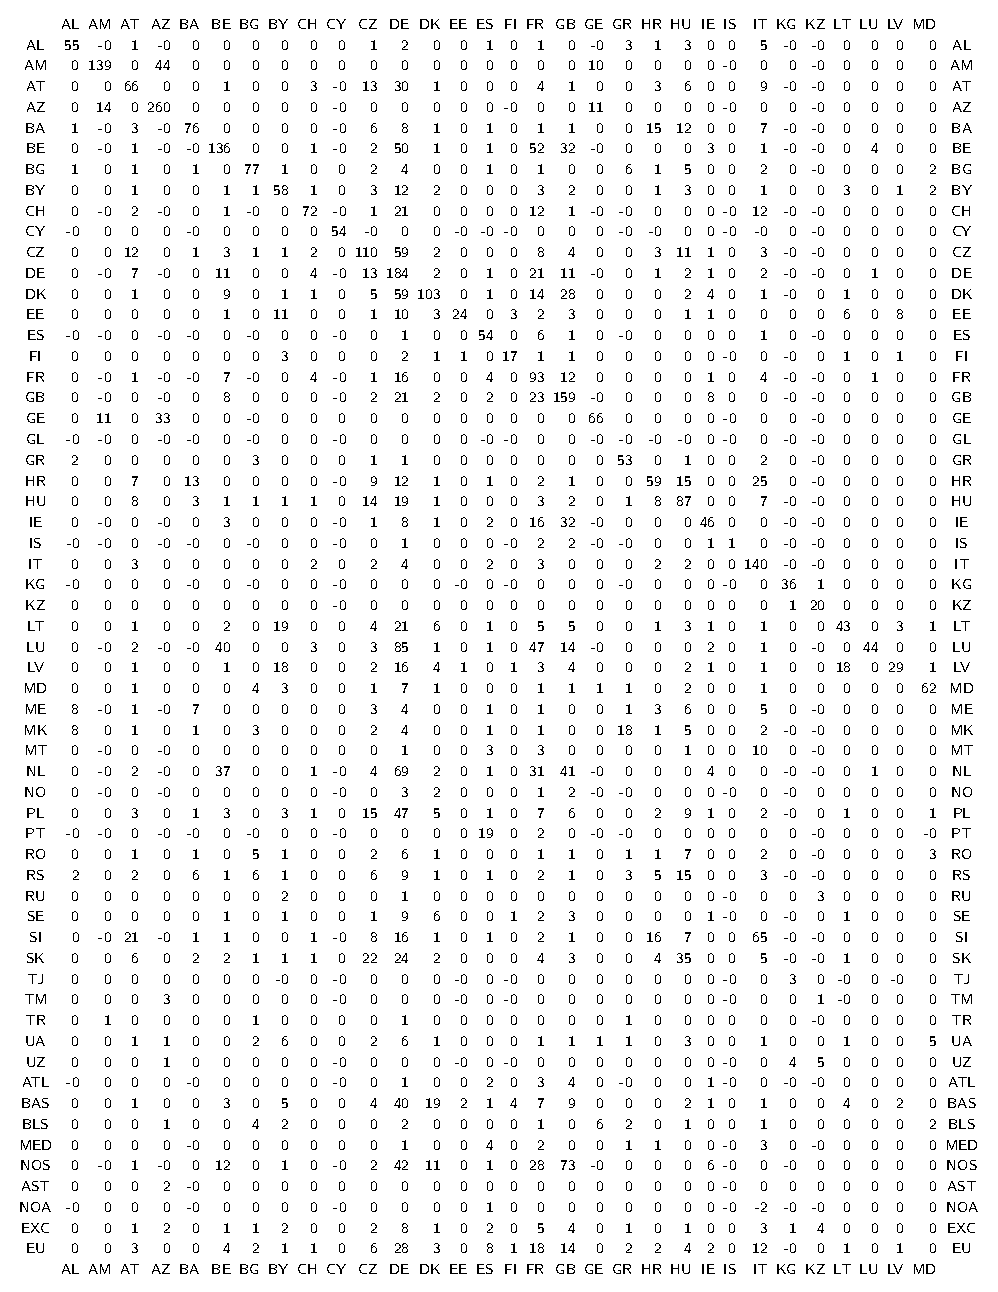
\epsfig{file=SR_Tables_2019/PM25_NH3_0.eps, width=\mywidth, height=\myheight}}\clearpage
\footnotesize{\mbox{Table \ref{ch:appx_sr2019}.11 Cont.: 2019 country-to-country blame matrices for \textbf{PM2.5}.}\\ Units: ng/m$^3$ per 15\% emis. red. of NH$_3$. \textbf{Emitters $\rightarrow$, Receptors $\downarrow$}. }\\[\baselineskip]\enlargethispage{\myenlarge} \hspace{-0.5cm} 
\centerline{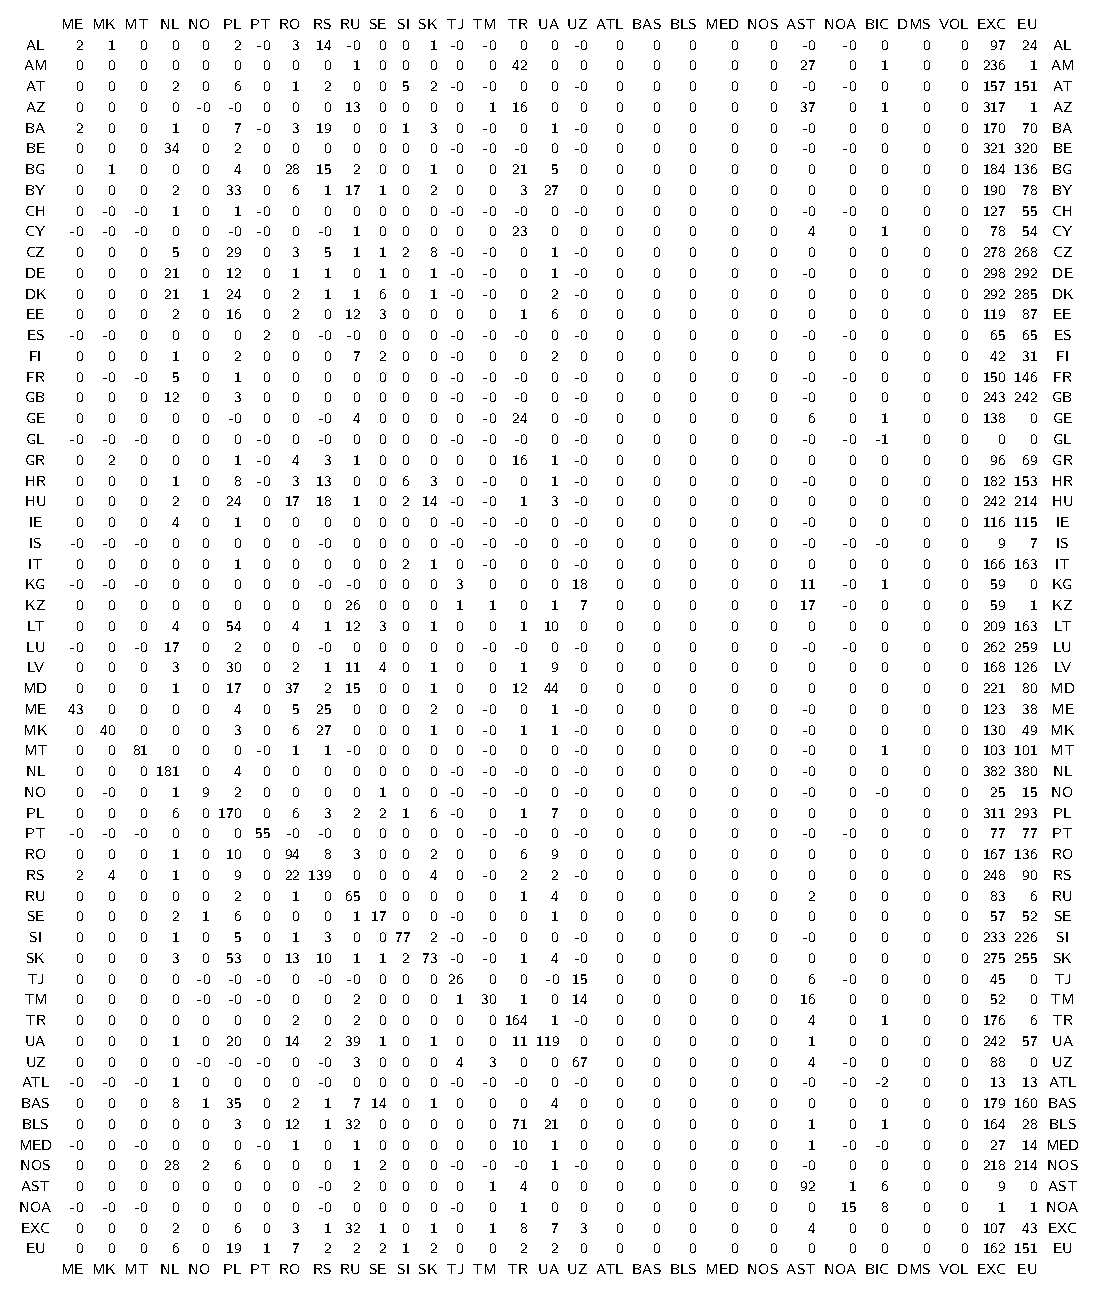
\epsfig{file=SR_Tables_2019/PM25_NH3_1.eps, width=\mywidth, height=\myheight}}\clearpage

% % table 12
\footnotesize{\mbox{Table \ref{ch:appx_sr2019}.12: 2019 country-to-country blame matrices for \textbf{PM2.5}.}\\ Units: ng/m$^3$ per 15\% emis. red. of VOC. \textbf{Emitters $\rightarrow$, Receptors $\downarrow$}. }\\[\baselineskip]\enlargethispage{\myenlarge} \hspace{-0.5cm} 
\centerline{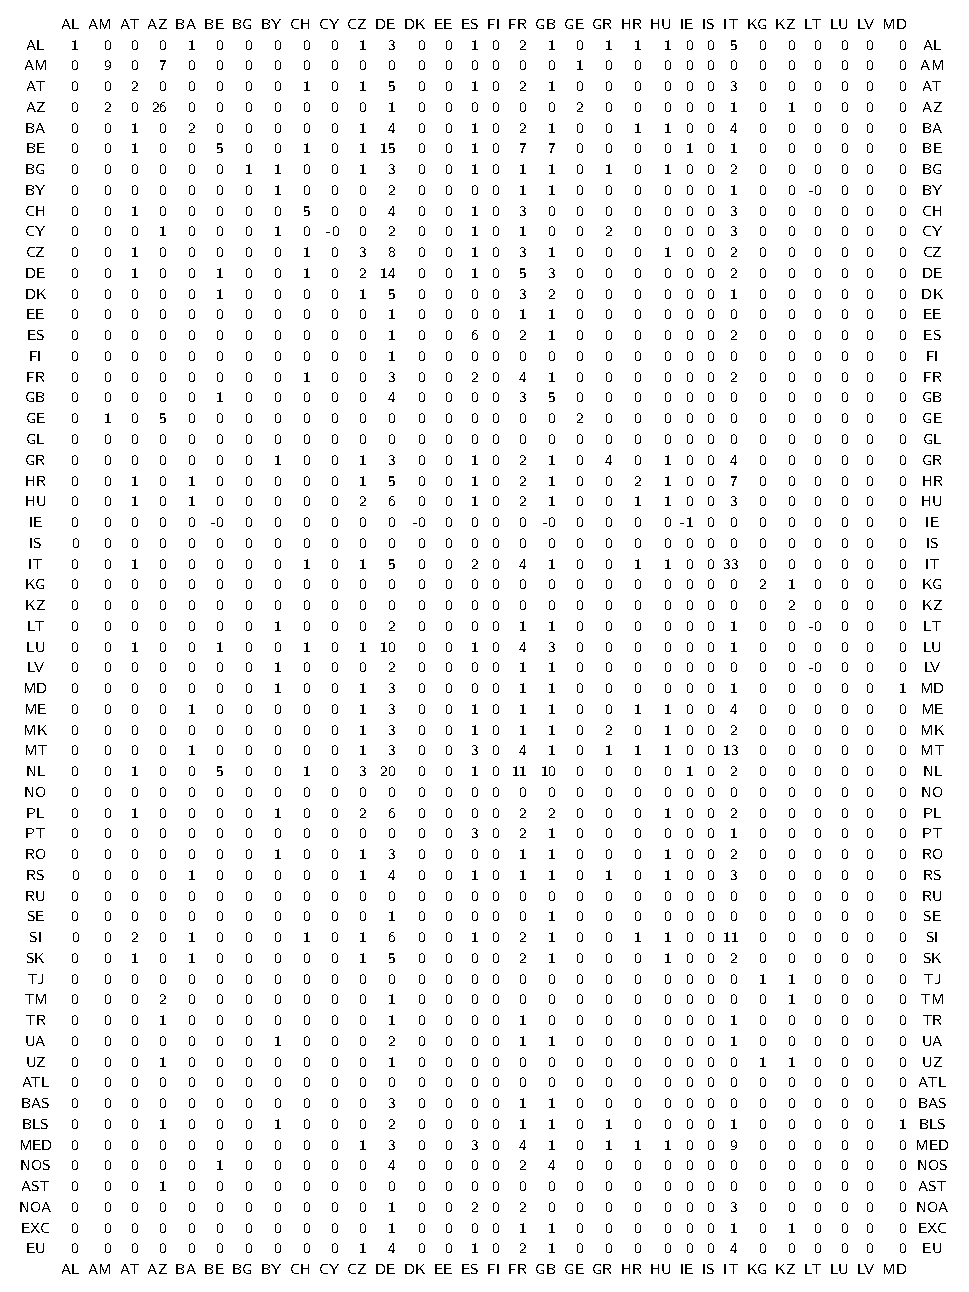
\epsfig{file=SR_Tables_2019/PM25_NMVOC_0.eps, width=\mywidth, height=\myheight}}\clearpage
\footnotesize{\mbox{Table \ref{ch:appx_sr2019}.12 Cont.: 2019 country-to-country blame matrices for \textbf{PM2.5}.}\\ Units: ng/m$^3$ per 15\% emis. red. of VOC. \textbf{Emitters $\rightarrow$, Receptors $\downarrow$}. }\\[\baselineskip]\enlargethispage{\myenlarge} \hspace{-0.5cm} 
\centerline{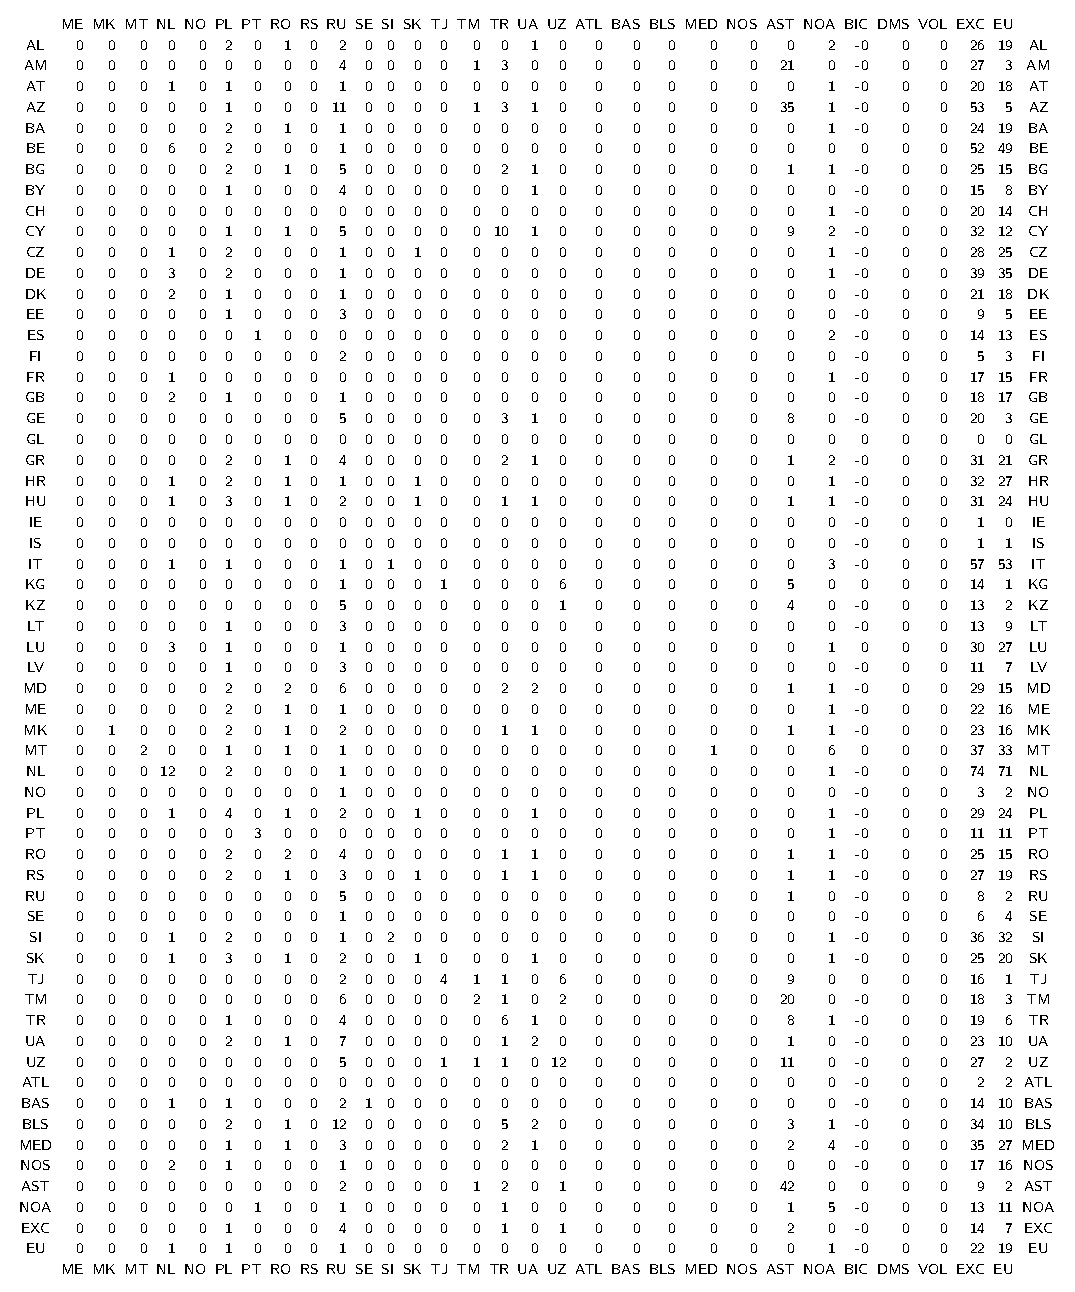
\epsfig{file=SR_Tables_2019/PM25_NMVOC_1.eps, width=\mywidth, height=\myheight}}\clearpage


% %table 13

\footnotesize{\mbox{Table \ref{ch:appx_sr2019}.13: 2019 country-to-country blame matrices for \textbf{PM2.5}.}\\ Units: ng/m$^3$ per 15\% emis. red. of PPM, SO$_x$, NO$_x$, NH$_3$ and VOC. \textbf{Emitters $\rightarrow$, Receptors $\downarrow$}. }\\[\baselineskip]\enlargethispage{\myenlarge} \hspace{-0.5cm} 
\centerline{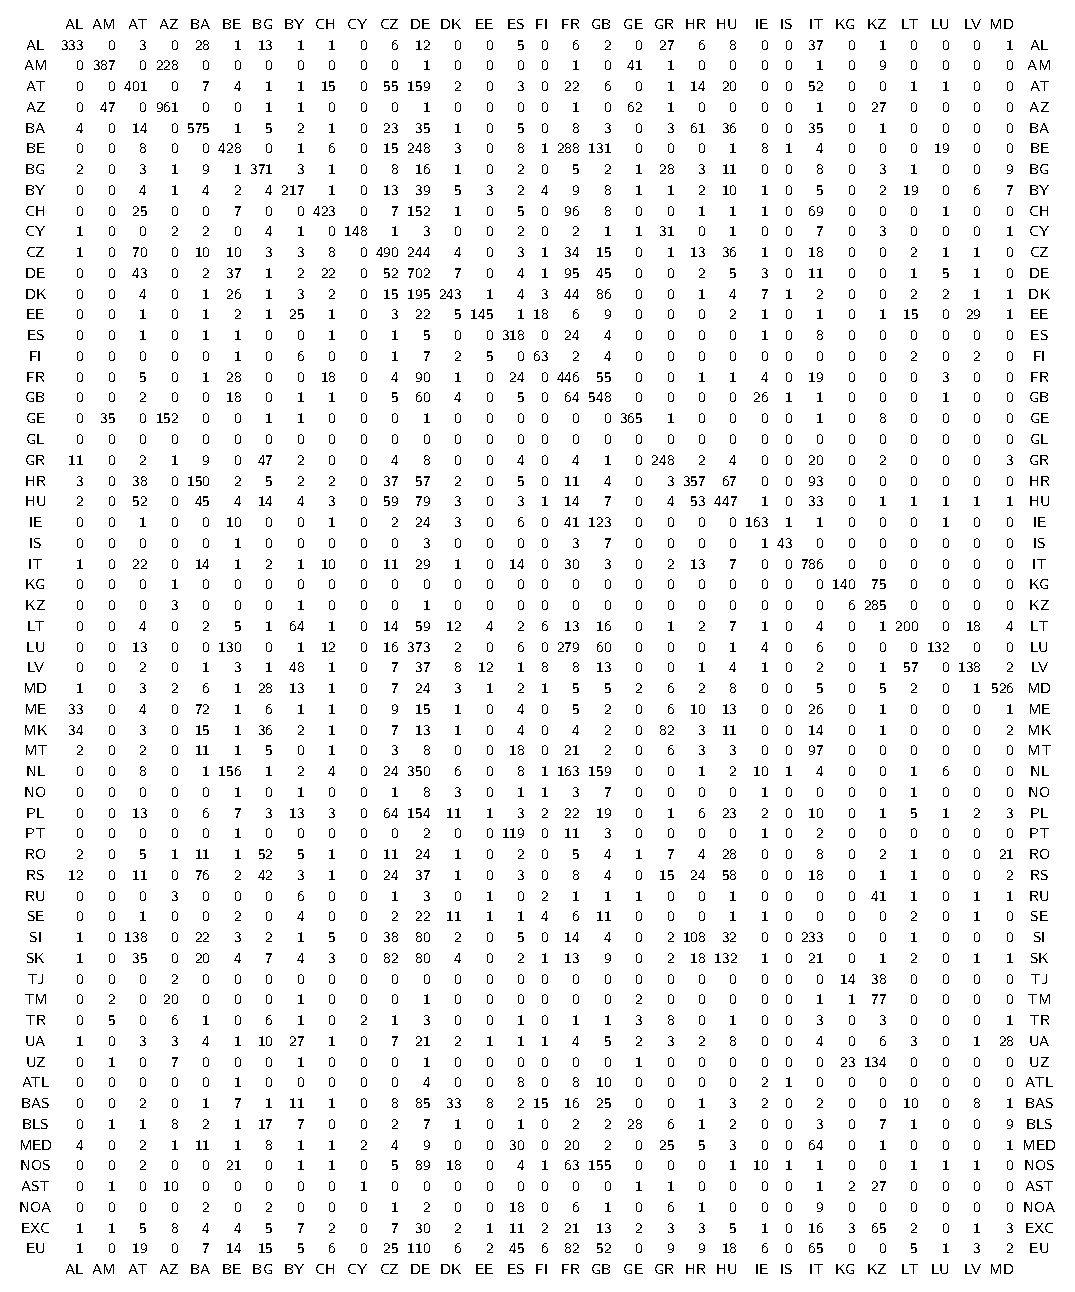
\epsfig{file=SR_Tables_2019/PM25_0.eps, width=\mywidth, height=\myheight}}\clearpage
\footnotesize{\mbox{Table \ref{ch:appx_sr2019}.13 Cont.: 2019 country-to-country blame matrices for \textbf{PM2.5}.}\\ Units: ng/m$^3$ per 15\% emis. red. of PPM, SO$_x$, NO$_x$, NH$_3$ and VOC. \textbf{Emitters $\rightarrow$, Receptors $\downarrow$}. }\\[\baselineskip]\enlargethispage{\myenlarge} \hspace{-0.5cm} 
\centerline{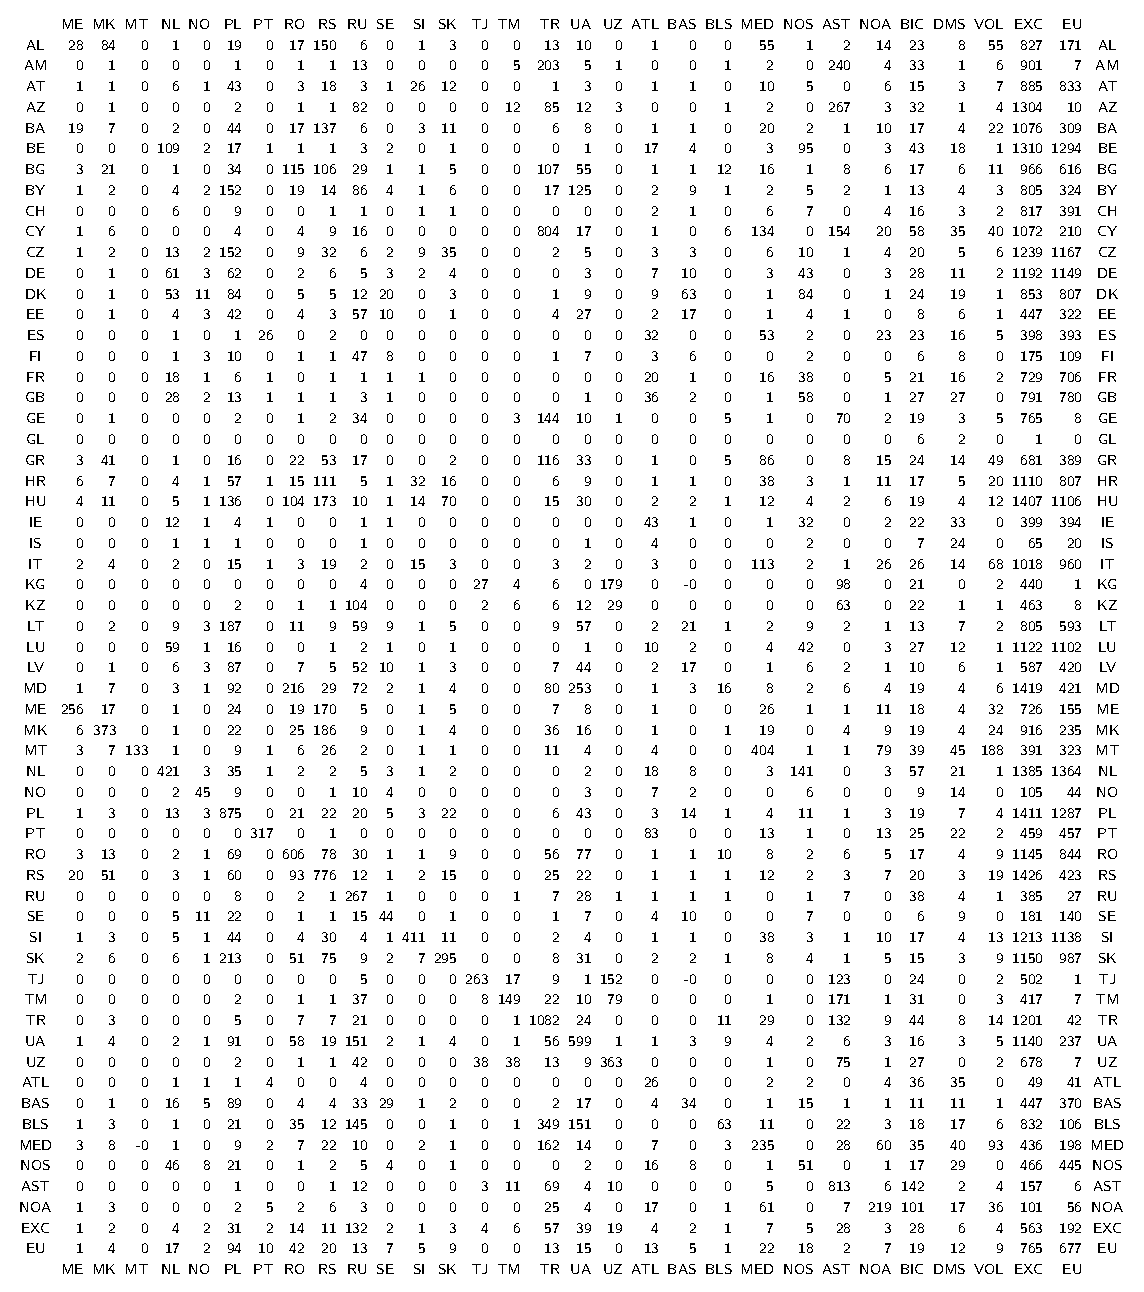
\epsfig{file=SR_Tables_2019/PM25_1.eps, width=\mywidth, height=\myheight}}\clearpage



% %table 14
 \footnotesize{\mbox{Table \ref{ch:appx_sr2019}.14: 2019
     country-to-country blame matrices for \textbf{fine EC}.}\\ Units:
   0.1 ng/m$^3$ per 15\% emis. red. of PPM. \textbf{Emitters $\rightarrow$, Receptors $\downarrow$}. }\\[\baselineskip]\enlargethispage{\myenlarge} \hspace{-0.5cm} 
 \centerline{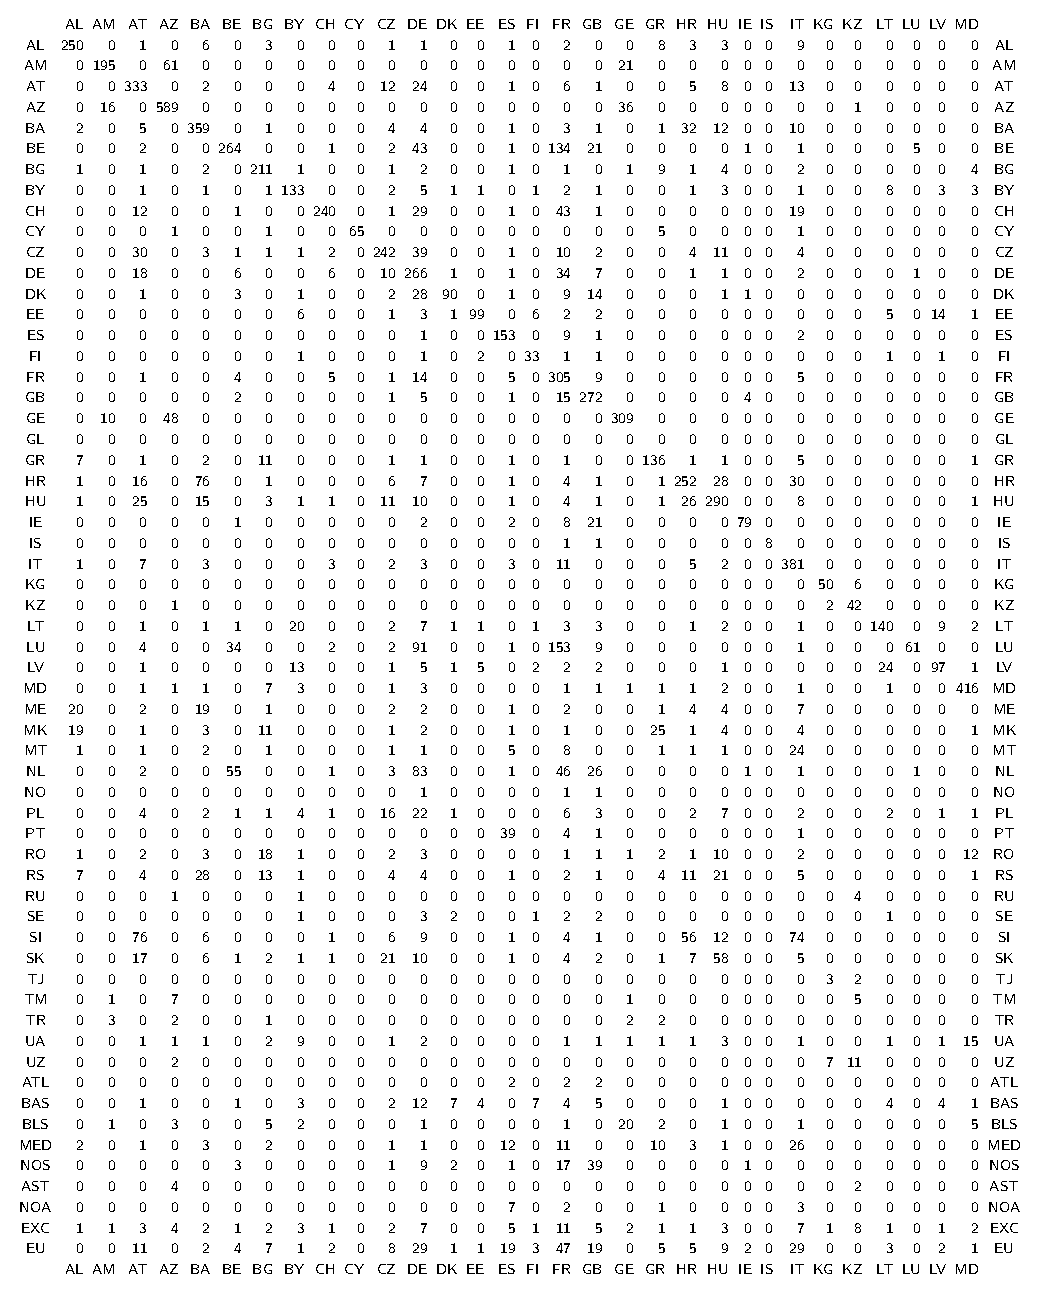
\epsfig{file=SR_Tables_2019/ECfine_0.eps, width=\mywidth, height=\myheight}}\clearpage
 \footnotesize{\mbox{Table \ref{ch:appx_sr2019}.14 Cont.: 2019
     country-to-country blame matrices for \textbf{fine EC}.}\\ Units:
   0.1 ng/m$^3$ per 15\% emis. red. of PPM. \textbf{Emitters $\rightarrow$, Receptors $\downarrow$}. }\\[\baselineskip]\enlargethispage{\myenlarge} \hspace{-0.5cm} 
 \centerline{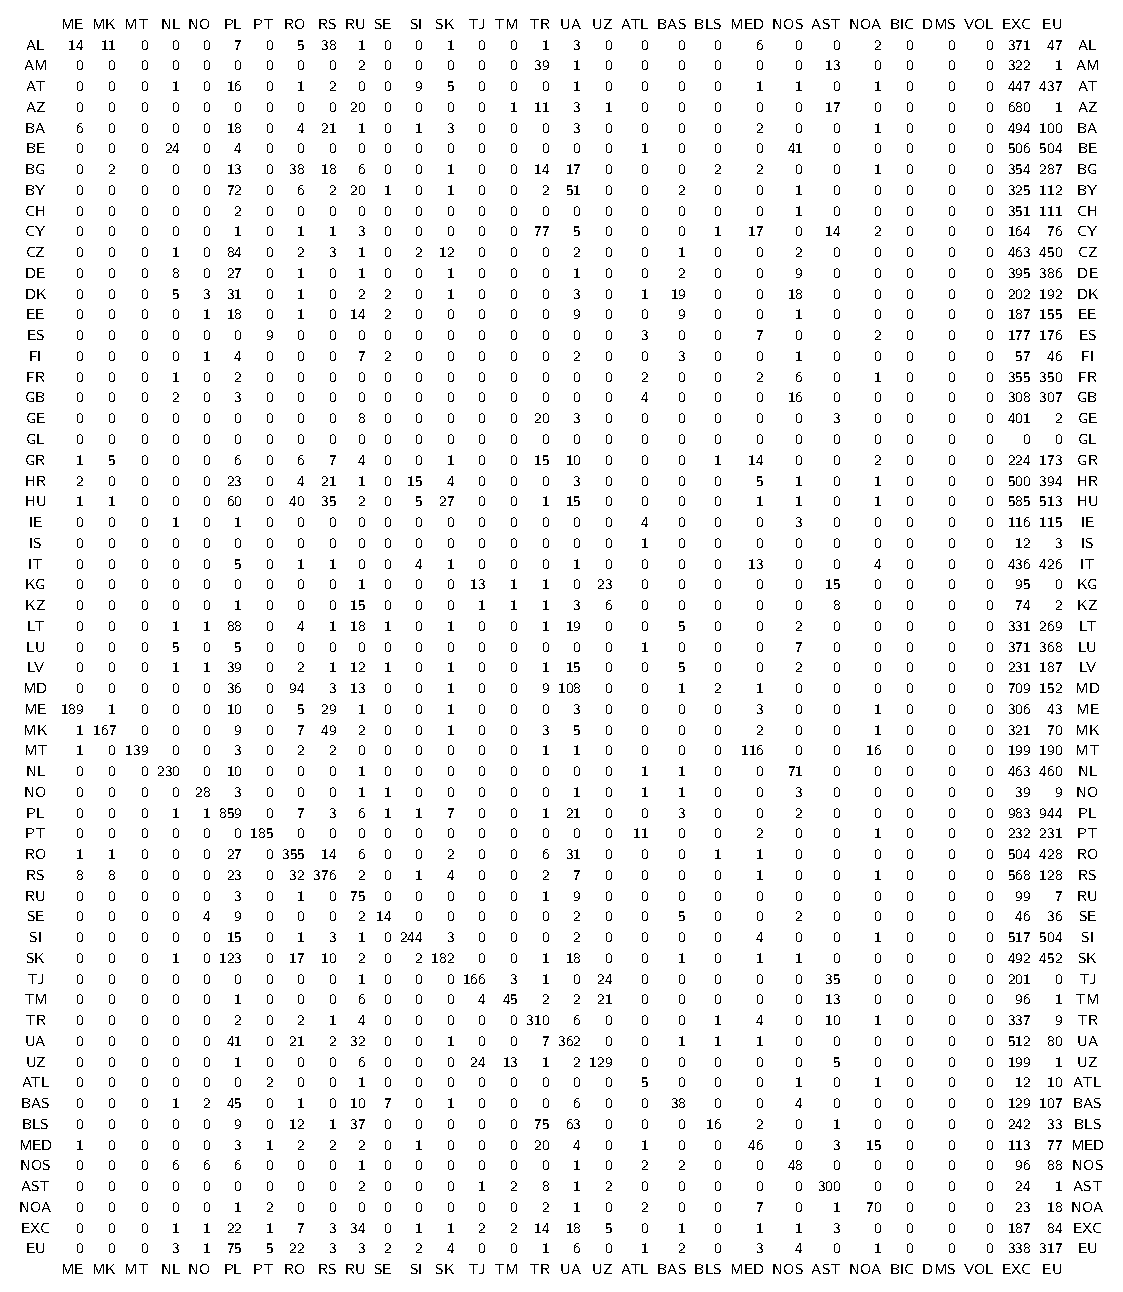
\epsfig{file=SR_Tables_2019/ECfine_1.eps,
     width=\mywidth, height=\myheight}}\clearpage



% %table 15
\footnotesize{\mbox{Table \ref{ch:appx_sr2019}.15: 2019
    country-to-country blame matrices for \textbf{coarse
      EC}.}\\ Units: 0.1 ng/m$^3$ per 15\% emis. red. of PPM. \textbf{Emitters $\rightarrow$, Receptors $\downarrow$}. }\\[\baselineskip]\enlargethispage{\myenlarge} \hspace{-0.5cm} 
\centerline{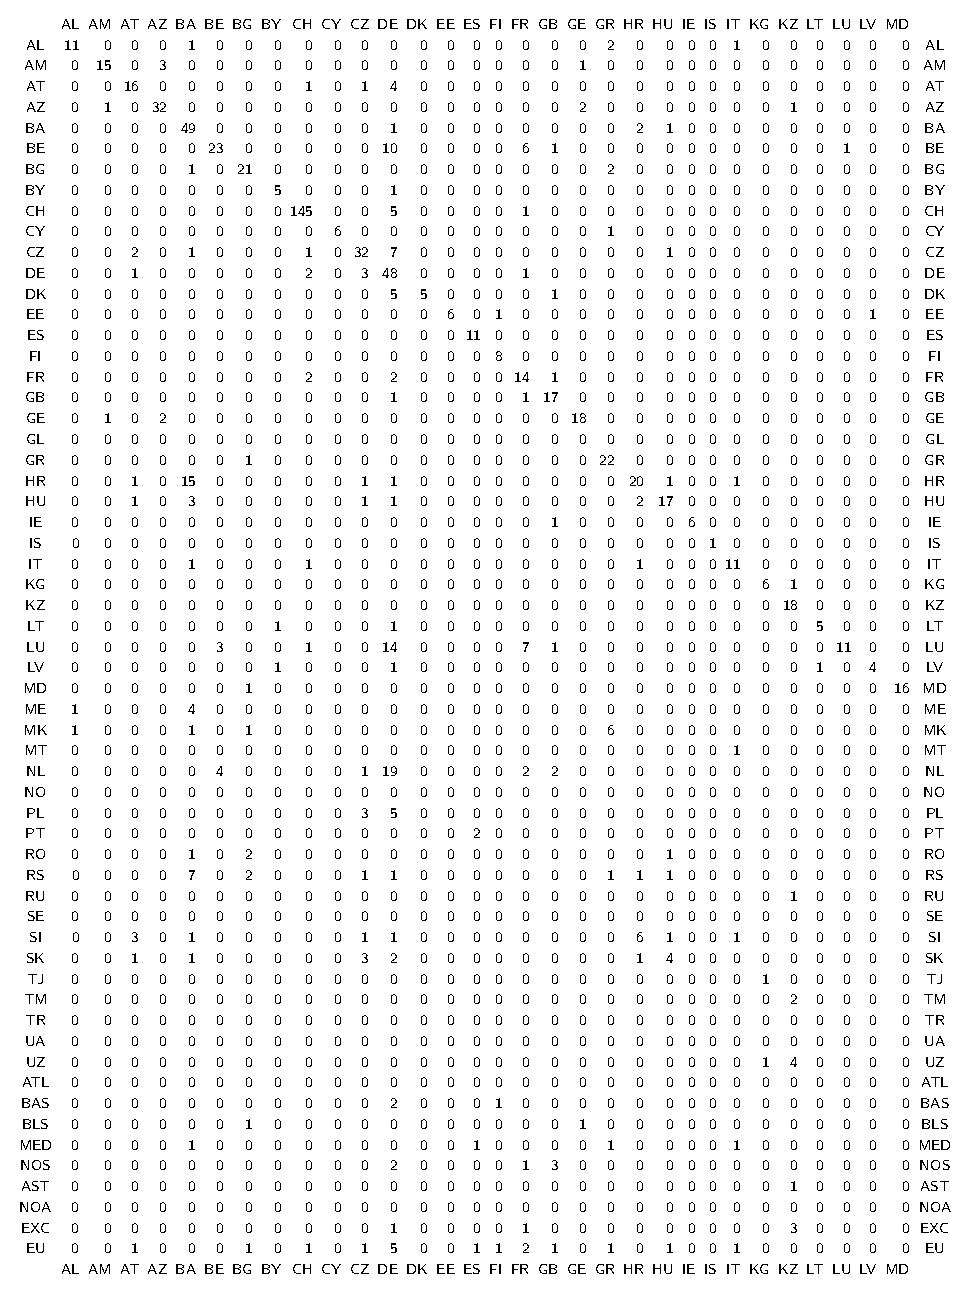
\epsfig{file=SR_Tables_2019/ECcoarse_0.eps, width=\mywidth, height=\myheight}}\clearpage
\footnotesize{\mbox{Table \ref{ch:appx_sr2019}.15 Cont.: 2019
    country-to-country blame matrices for \textbf{coarse
      EC}.}\\ Units: 0.1 ng/m$^3$ per 15\% emis. red. of PPM. \textbf{Emitters $\rightarrow$, Receptors $\downarrow$}. }\\[\baselineskip]\enlargethispage{\myenlarge} \hspace{-0.5cm} 
\centerline{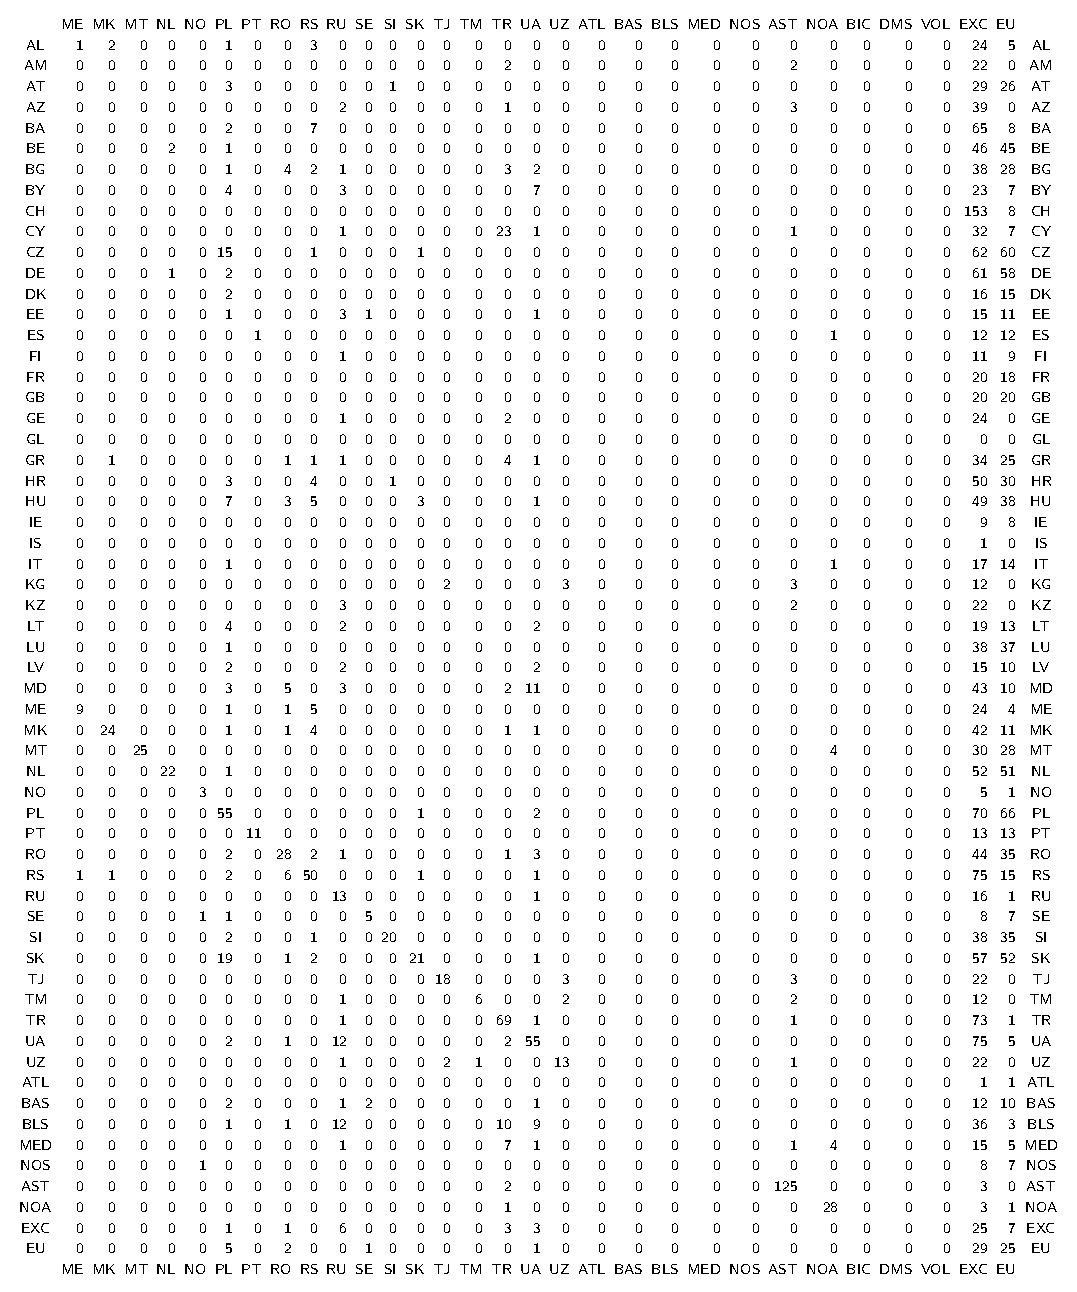
\epsfig{file=SR_Tables_2019/ECcoarse_1.eps,
    width=\mywidth, height=\myheight}}\clearpage


% %table 16

\footnotesize{\mbox{Table \ref{ch:appx_sr2019}.16: 2019 country-to-country blame matrices for \textbf{PPM2.5}}\\ Units: ng/m$^3$ per 15\% emis. red. of PPM. \textbf{Emitters $\rightarrow$, Receptors $\downarrow$}. }\\[\baselineskip]\enlargethispage{\myenlarge} \hspace{-0.5cm} 
\centerline{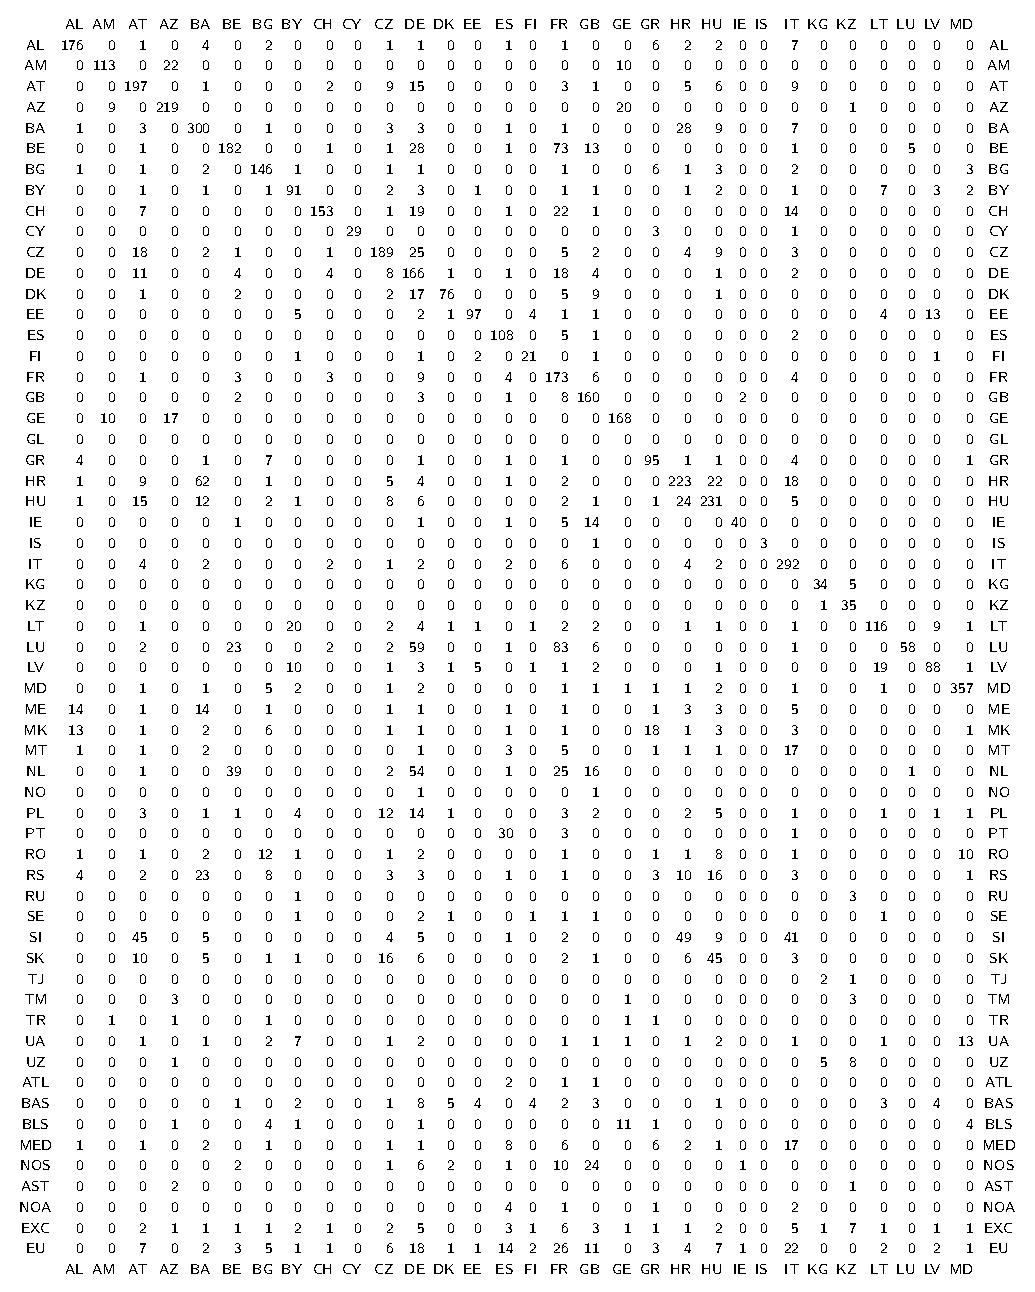
\epsfig{file=SR_Tables_2019/PPM25_0.eps, width=\mywidth, height=\myheight}}\clearpage
\footnotesize{\mbox{Table \ref{ch:appx_sr2019}.16 Cont.: 2019 country-to-country blame matrices for \textbf{PPM2.5}}\\ Units: ng/m$^3$ per 15\% emis. red. of PPM. \textbf{Emitters $\rightarrow$, Receptors $\downarrow$}. }\\[\baselineskip]\enlargethispage{\myenlarge} \hspace{-0.5cm} 
\centerline{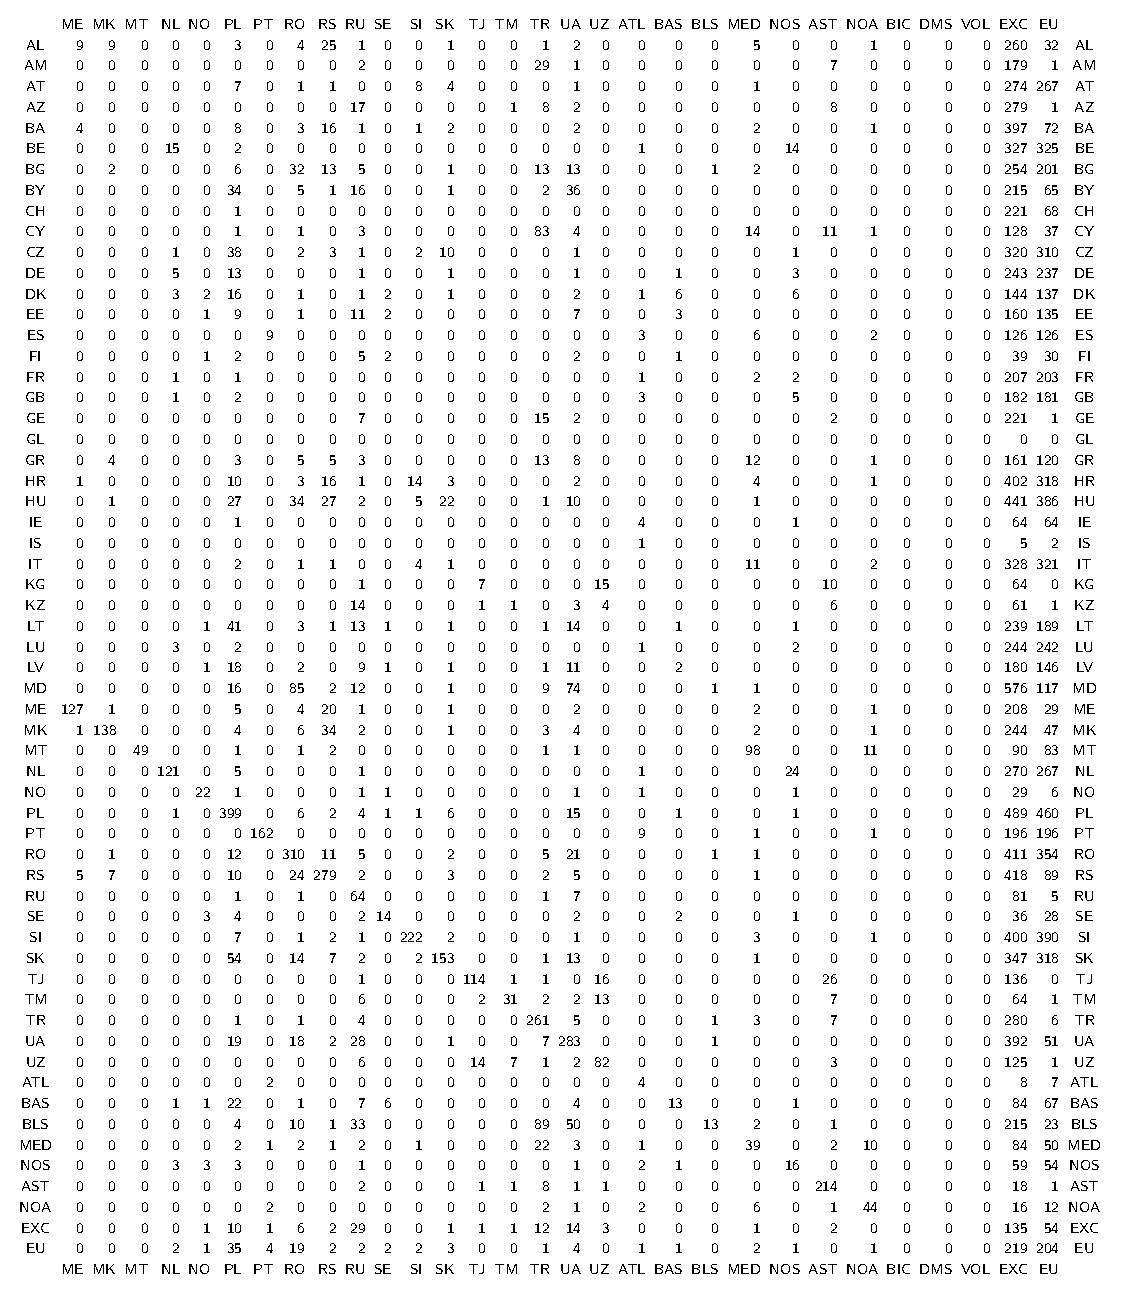
\epsfig{file=SR_Tables_2019/PPM25_1.eps, width=\mywidth, height=\myheight}}\clearpage




%put back old parindent and headsep value
\setlength{\parindent}{\previousparindent}
\setlength{\headsep}{\previousheadsep}

% to 'recover' from the SR table's footnotesize
\normalsize

\cleardoublepage

%%% Local Variables: 
%%% mode: latex
%%% TeX-master: "report"
%%% End: 
